\documentclass[fontsize=12pt,paper=a4,twoside,bibtotoc,idxtotoc,
liststotoc,pagesize,BCOR1.2cm,DIV15,chapterprefix,pagesize=pdftex]{scrbook}

%\usepackage[utf8x]{inputenc}
\usepackage[ngerman]{babel}
\usepackage{amsmath}
\usepackage{amssymb}
\usepackage{dsfont}
\usepackage{textcomp}
\usepackage{stmaryrd}
\usepackage{graphicx}
\usepackage{xcolor}
\usepackage{tikz}

\title{Einführung in Sage}
\author{Dr.Jochen Schulz}
\date{10-10-11}


%\usepackage{fontspec,xunicode}
% %\usepackage{polyglossia}
%\setdefaultlanguage[spelling=new, latesthyphen=true]{german}
%\setsansfont{DejaVu Sans}
%\setsansfont{Verdana}
%\setsansfont{Arial}
%\setromanfont[Mapping=tex-text]{Linux Libertine}
%\setsansfont[Mapping=tex-text]{Myriad Pro}
%\setmonofont[Mapping=tex-text]{Courier New}

%\setsansfont{Linux Biolinum}

\usepackage[ngerman]{babel}
\selectlanguage{ngerman}

%
% math/symbols
%
\usepackage{amssymb}
\usepackage{amsthm}
% \usepackage{latexsym}
\usepackage{amsmath}
%\usepackage{amsxtra} %Weitere Extrasymbole
%\usepackage{empheq} %Gleichungen hervorheben
%\usepackage{bm}
 %\bm{A} Boldface im Mathemodus
\usepackage{fontspec,xunicode,xltxtra}

\usepackage{multimedia}
%\usepackage{tikz}

\usepackage{cellspace}
\setlength{\cellspacetoplimit}{2pt}
\setlength{\cellspacebottomlimit}{2pt}

%%%%%%%%%%%%%%%%%% Fuer Frames [fragile]-Option verwenden!
%Programm-Listing
%%%%%%%%%%%%%%%%%%
%Listingsumgebung fuer verbatim
%Grauhinterlegeter Text
%Automatischer Zeilenumbruch ist aktiviert
%\usepackage{listings}
\usepackage[framed]{mcode}
%\usepackage{mcode}
% This command allows you to typeset syntax highlighted Matlab
% code ``inline''.
% mcode fuer matlab

\definecolor{lgray}{gray}{0.80}
\definecolor{gray}{gray}{0.3}
\definecolor{darkgreen}{rgb}{0,0.4,0}
\definecolor{darkblue}{rgb}{0,0,0.8}
\definecolor{key}{rgb}{0,0.5,0} 
\definecolor{NU0}{RGB}{68,85,136} % #458
\definecolor{KW3}{RGB}{85,68,136}
\definecolor{KW4}{RGB}{153,0,0}
\definecolor{dred}{RGB}{221,17,68} % #d14
\definecolor{BG}{RGB}{240,240,240}
%\lstset{backgroundcolor=\color{lgray}, frame=single, basicstyle=\ttfamily, breaklines=true}
%\lstnewenvironment{sage}{\lstset{,language=python, keywordstyle=color{blue},    commentstyle=color{green}, emphstyle=\color{red}, %frame=single, stringstyle=\color{red}, basicstyle=\ttfamily, ,mathescape =true,escapechar=§}}{}

\lstdefinelanguage{fooHaskell} {%
  basicstyle=\footnotesize\ttfamily,%
  commentstyle=\slshape\color{gray},%
  keywordstyle=\bfseries,%\color{KW4},
  breaklines=true,
  sensitive=true,
  xleftmargin=1pc,
  emph={[1]
    FilePath,IOError,abs,acos,acosh,all,and,any,appendFile,approxRational,asTypeOf,asin,
    asinh,atan,atan2,atanh,basicIORun,break,catch,ceiling,chr,compare,concat,concatMap,
    const,cos,cosh,curry,cycle,decodeFloat,denominator,digitToInt,div,divMod,drop,
    dropWhile,either,elem,encodeFloat,enumFrom,enumFromThen,enumFromThenTo,enumFromTo,
    error,even,exp,exponent,fail,filter,flip,floatDigits,floatRadix,floatRange,floor,
    fmap,foldl,foldl1,foldr,foldr1,fromDouble,fromEnum,fromInt,fromInteger,fromIntegral,
    fromRational,fst,gcd,getChar,getContents,getLine,head,id,inRange,index,init,intToDigit,
    interact,ioError,isAlpha,isAlphaNum,isAscii,isControl,isDenormalized,isDigit,isHexDigit,
    isIEEE,isInfinite,isLower,isNaN,isNegativeZero,isOctDigit,isPrint,isSpace,isUpper,iterate,
    last,lcm,length,lex,lexDigits,lexLitChar,lines,log,logBase,lookup,map,mapM,mapM_,max,
    maxBound,maximum,maybe,min,minBound,minimum,mod,negate,not,notElem,null,numerator,odd,
    or,ord,otherwise,pi,pred,primExitWith,print,product,properFraction,putChar,putStr,putStrLn,quot,
    quotRem,range,rangeSize,read,readDec,readFile,readFloat,readHex,readIO,readInt,readList,readLitChar,
    readLn,readOct,readParen,readSigned,reads,readsPrec,realToFrac,recip,rem,repeat,replicate,return,
    reverse,round,scaleFloat,scanl,scanl1,scanr,scanr1,seq,sequence,sequence_,show,showChar,showInt,
    showList,showLitChar,showParen,showSigned,showString,shows,showsPrec,significand,signum,sin,
    sinh,snd,span,splitAt,sqrt,subtract,succ,sum,tail,take,takeWhile,tan,tanh,threadToIOResult,toEnum,
    toInt,toInteger,toLower,toRational,toUpper,truncate,uncurry,undefined,unlines,until,unwords,unzip,
    unzip3,userError,words,writeFile,zip,zip3,zipWith,zipWith3,listArray,doParse
  },%
  emphstyle={[1]\color{NU0}},%
  emph={[2]
    Bool,Char,Double,Either,Float,IO,Integer,Int,Maybe,Ordering,Rational,Ratio,ReadS,Show,ShowS,String,
    Word8,InPacket
  },%
  emphstyle={[2]\bfseries\color{KW4}},%
  emph={[3]
    case,class,data,deriving,do,else,if,import,in,infixl,infixr,instance,let,
    module,of,primitive,then,type,where
  },
  emphstyle={[3]\color{darkblue}},
  emph={[4]
    quot,rem,div,mod,elem,notElem,seq
  },
  emphstyle={[4]\color{NU0}\bfseries},
  emph={[5]
    EQ,False,GT,Just,LT,Left,Nothing,Right,True,Show,Eq,Ord,Num
  },
  emphstyle={[5]\color{KW4}\bfseries},
  morestring=[b]",%
  morestring=[b]',%
  stringstyle=\color{darkgreen},%
  showstringspaces=false
}
\lstnewenvironment{hs}
{\lstset{language=fooHaskell,backgroundcolor=\color{BG}}}
{\smallskip}
\newcommand{\ihs}[1]{\lstset{language=fooHaskell,basicstyle=\color[gray]{0.6}}\lstinline|#1|}


\lstdefinelanguage{fooMatlab} {%
backgroundcolor=\color[gray]{0.9},
breaklines=true,
basicstyle=\ttfamily\small,
%otherkeywords={ =},
%keywordstyle=\color{blue},
%stringstyle=\color{darkgreen},
showstringspaces=false,
%emph={for, while, if, elif, else, not, and, or, printf, break, continue, return, end, function},
%emphstyle=\color{blue},
%emph={[2]True, False, None, self, NaN, NULL},
%emphstyle=[2]\color{key},
%emph={[3]from, import, as},
%emphstyle=[3]\color{blue},
%upquote=true,
%morecomment=[s]{"""}{"""},
%commentstyle=\color{gray}\slshape,
%framexleftmargin=1mm, framextopmargin=1mm, 
%title=\tiny matlab,
frame=single,
%mathescape =true,
%escapechar=§
}
\newcommand{\imatlab}[1]{\lstset{language=fooMatlab,basicstyle=\color[gray]{0.6}}\lstinline|#1|}
\lstnewenvironment{matlab}[1][]{\lstset{language=fooMatlab,xleftmargin=0.2cm,frame=none,backgroundcolor=\color{white},basicstyle=\color{darkblue}\ttfamily\small,#1}}{} 
\lstnewenvironment{matlabin}[1][]{\lstset{language=fooMatlab,#1}}{} 
\newcommand{\matinput}[1]{\lstset{language=fooMatlab}\lstinputlisting{#1}}

\lstdefinelanguage{fooPython} {%
language=python,
backgroundcolor=\color[gray]{0.7},
breaklines=true,
basicstyle=\ttfamily\small,
%otherkeywords={ =},
keywordstyle=\color{blue},
stringstyle=\color{darkgreen},
morestring=[b]",%
morestring=[b]',%
showstringspaces=false,
emph={class, pass, in, for, while, if, is, elif, else, not, and, or,
def, print, exec, break, continue, return, import, from, lambda, null},
emphstyle=\color{blue},
emph={[2]True, False, None, self},
emphstyle=[2]\color{key},
emph={[3]from, import, as},
emphstyle=[3]\color{blue},
upquote=true,
morecomment=[s]{"""}{"""},
comment=[l]{\#},
commentstyle=\color{gray},
%framexleftmargin=1mm, framextopmargin=1mm, 
%title=\tiny python,
%caption=python,
frame=single
%frameround=tttt,
%mathescape =true,
%escapechar=§
}

\newcommand{\pyinput}[1]{\lstset{language=fooPython}\lstinputlisting{#1}}
\newcommand{\isage}[1]{{\lstset{language=fooPython,basicstyle=\color[gray]{0.3}}\lstinline|#1|}}

\lstnewenvironment{pyout}[1][]{\lstset{language=fooPython,xleftmargin=0.2cm,frame=none,backgroundcolor=\color{white},basicstyle=\color{darkblue}\ttfamily\small,#1}}{}
\lstnewenvironment{pyin}[1][]{\lstset{language=fooPython,#1}}{}
\lstnewenvironment{sageout}[1][]{\lstset{language=fooPython,xleftmargin=0.2cm,frame=none,backgroundcolor=\color{white},basicstyle=\color{darkblue}\ttfamily\small,#1}}{}
\lstnewenvironment{sagein}[1][]{\lstset{language=fooPython,#1}}{}

%\usepackage{caption}
%\DeclareCaptionFont{white}{ \color{white} }
%\DeclareCaptionFormat{listing}{
%  \colorbox[cmyk]{0.43, 0.35, 0.35,0.01 }{
%      \parbox{\textwidth}{\hspace{15pt}#1#2#3}
%        }
%        }
%        \captionsetup[lstlisting]{ format=listing, labelfont=white, textfont=white, singlelinecheck=false, margin=0pt, font={bf,footnotesize} }


\usepackage{mydef}
%\usepackage{cmap} % you can search in the pdf for umlauts and ligatures
\usepackage{colonequals} %corrects the definition-symbols \colonequals (besides others)

\usepackage{ifthen}

%%%%%%%%%%%%%%%%%%%
%Neue Definitionen
%%%%%%%%%%%%%%%%%%%

%Newcommands
\newcommand{\Fun}[1]{\mathcal{#1}}      %Mathcal fuer Funktoren
\newcommand{\field}[1]{\mathbb{#1}}     %Grundkoerper ?? in mathds

\newcommand{\A}{\field{A}}              %Affines A
\newcommand{\Fp}{\field{F}_{\!p}}       %Endlicher Koerper mit p Elementen
\newcommand{\Fq}{\field{F}_{\!q}}       %Endlicher Koerper mit q Elementen
\newcommand{\Ga}{\field{G}_{a}}         %Add Gruppenschema
\newcommand{\K}{\field{K}}              %Generischer Koerper 
\newcommand{\N}{\field{N}}              %Nat Zahlen
\newcommand{\Pj}{\field{P}}             %Projektives P
\newcommand{\R}{\field{R}} 		%Reelle Zahlen
\newcommand{\Q}{\field{Q}}              %Rationale Zahlen  
\newcommand{\Qt}{\field{H}}             %Quaternionen 
\newcommand{\V}{\field{V}}              %Vektorbuendel V
\newcommand{\Z}{\field{Z}}              %Ganze Zahlen
\DeclareMathOperator{\Real}{Re}

\newcommand{\fdg}{\;|\;}                 %fuer die gilt

%Operatoren
\DeclareMathOperator{\Abb}{Abb}
%\usepackage{sagetex}


%
% Aufgaben
%
\parindent0cm % Abs�tze nicht einr�cken 
% Definieren einer neuen Farbe
\definecolor{light-gray}{gray}{.9}

\newcounter{zaehler}     % neuen Z�hler einf�hren
\newenvironment{aufgn}[2][0]
%---- Header
{\begin{samepage}%
%\colorbox{light-gray}{%                         % Box in gray
% \makebox[\textwidth]{%                           % Box in linewidth
%\textbf{Aufgabe \arabic{zaehler} } }\hspace{-\textwidth}\makebox[\textwidth]{\hfill #1 Punkte} }\\[0.05cm]       % Header
\dotfill\\
{\large\textbf{Aufgabe \arabic{zaehler} \ifthenelse{ \equal{#2}{} }{}{: \emph{ #2 } }}\ifthenelse{-1=#1}{(testierbar)}{}\ifthenelse{0=#1 \or -1=#1}{}{\hfill #1 Punkte} }\\[0.4cm]
%{\large\textbf{Exercise \arabic{zaehler}  #2 }\ifthenelse{-1=#1}{(testierbar)}{}\ifthenelse{0=#1 \or -1=#1}{}{\hfill #1 Punkte} }\\[0.4cm]
\begin{minipage}{\textwidth}%
}%
%-----  foot
{\end{minipage}\nopagebreak%\begin{minipage}{1cm} \end{minipage}
%\\ 
%\begin{minipage}{0.1cm} \end{minipage} 
%\hrulefill \begin{minipage}{1cm} \end{minipage}\\[1cm]  
\stepcounter{zaehler}                           % increase counter
\end{samepage}%
\\%
\bigskip%
}


\newenvironment{aufg}[1][0]
%---- Header
{\begin{samepage}%
\refstepcounter{zaehler}% increase counter
%\colorbox{light-gray}{%                         % Box in gray
% \makebox[\textwidth]{%                           % Box in linewidth
%\textbf{Aufgabe \arabic{zaehler} } }\hspace{-\textwidth}\makebox[\textwidth]{\hfill #1 Punkte} }\\[0.05cm]       % Header
\dotfill\\
{\large\textbf{Aufgabe \arabic{zaehler} }\ifthenelse{-1=#1}{(testierbar)}{}\ifthenelse{0=#1 \or -1=#1}{}{\hfill #1 Punkte} }\\[0.4cm]
\begin{minipage}{\textwidth}%
}%
%-----  foot
{\end{minipage}\nopagebreak%\begin{minipage}{1cm} \end{minipage}
%\\ 
%\begin{minipage}{0.1cm} \end{minipage} 
%\hrulefill \begin{minipage}{1cm} \end{minipage}\\[1cm]  
\end{samepage}%
\\%
\bigskip%
}

\begin{document}
\maketitle
\tableofcontents

%%%%%%%%%%%%%%%%%%%%%%%%%%%%%%%%%%%%%%
\chapter{Einleitung}
\section{Was ist Sage?}
%\subsection{Was ist Sage?}
%%%%%%%%%%%%%%%%%%%%%%%%%%%%%%%%%%%%%%

Sage ist ein pythonbasiertes, objektorientiertes Open-source (GPL) Mathematik Software System, dass es seit dem 24. Februar 2005 gibt.
In Sage findet man eine Alternative zu den 4 M's: Magma, Maple, Mathematica, Matlab.\newline
Das (Haupt-)Interface ist der Browser, dennoch besitzt Sage Frontends für viele externe Software.\newline
Zu den Stärken von Sage zählt sicherlich, dass es viele andere CAS und Libraries unter einer einheitlichen Oberfl\"ache vereint 
(so z.B. Maxima, Pari, GAP, R, Magma, ...), sowie durch Python eine sehr mächtige Programmiersprache als Grundlage hat. Desweiteren 
ist der Source Code offen, es gibt ein umfangreiches Hilfesystem sowie viele freie Materialien im Internet.\newline
Wie alles, so hat auch Sage trotz seiner vielen Stärken auch Schwächen, so ist der Befehlsumfang nicht so mächtig, wie der von Maple,Mthematica 
oder Matlab; außerdem fehlt eine standalone Entwicklungsumgebung. Als Alternative zum Webinterface findet sich Cantor.

%%%%%%%%%%%%%%%%%%%%%%%%%%%%%%%%%%%%%%
\subsection{Vorab}
%%%%%%%%%%%%%%%%%%%%%%%%%%%%%%%%%%%%%%

Sage incl. online Testversion und gratis Download sowie einigen anderen Features findet sich unter http://www.sagemath.org/.\newline
Hier ein paar grundlegende Tipps, Tricks und Dinge, die einfach beherzigt werden sollten:\newline
\begin{itemize}
 \item Mehrere Befehle in einer Zeile durch {\color{blue} \verb~;~} trennen. 
 \item Bei Eingaben, die über mehrere Zeilen gehen, kann ein
  Zeilenumbruch durch {\color{blue} \verb~<ENTER>~} erreicht werden.
 \item Das Auswerten eines Blocks erfolgt mit {\color{blue} \verb~<SHIFT>+<ENTER>~}.
 \item Ein neues Eingabefeld erhält man durch klicken auf den blauen, horizontalen Balken
 \item {\color{blue} \isage{_} } refenziert die letzte Ausgabe.
 \item Löschen aller eigenen Variablen und Zurücksetzen auf den Anfangsstatus: {\color{blue} \isage{reset()}}
%\item Anzeigen aller definierten Variablen: {\color{blue} anames(All)}
%\item Anzeigen aller selbst definierten Variablen: {\color{blue} anames(All,User)}
 \item Das Feld aktivieren von \emph{Typeset} lässt alle Ausgaben von \LaTeX{} rendern.
%\item profiler und debugger -> commandline
 \item Html- und/oder \LaTeX-Dokumentation:{\color{blue} \verb~<SHIFT>+<KLICK>~ }auf den blauen Balken
%\item Publish: Im Notebook kann durch klicken des \alert{Publish}-Reiters das Notebook für alle offen gelegt werden. 
%\item Unter dem Menupunkt \alert{File} kann man 
 \item {\color{blue} Autocompletion :} mit der {\color{blue} \verb~<TAB>~}-Taste erhält man alle möglichen Funktions- und/oder Variablen-Namen im gegebenen Kontext.\\
  Dies gilt insbesondere auch für Objektfunktionen (\isage{object.function()})
 \item {\color{blue} \isage{<command>?} :} gibt ausführliche Hilfe zu \isage{command} an.
 \item {\color{blue} \isage{help(<command>)} :} öffnet ein Hilfefenster zu \isage{command}.
 \item online Dokumentation:
  \begin{itemize}
   \item Sage: http://www.sagemath.org/doc/index.html
   \item Python: http://docs.python.org/
  \end{itemize}
\end{itemize}
\newpage

%%%%%%%%%%%%%%%%%%%%%%%%%%%%%%%%%%%%%%
\section{Überblick}
%%%%%%%%%%%%%%%%%%%%%%%%%%%%%%%%%%%%%%

Als Einstieg und kleine Motivation, wofür man Sage einsetzen kann, wollen wir erst einmal ein paar grundlegende Operationen 
vorstellen:
\begin{itemize}
 \item Deklarieren von Variablen mir \isage{var()}, z.B.{\verb~var('a')~} 
 \item Definieren von Variablen mit {\color{blue}'='}, z.B. {\verb~a=3~} 
 \item Definieren von Funktionen mit{\color{blue} '='}, z.B. {\verb~f(x) = x^2 - 6*x~}
 \item Grenzwertbestimmung: {\color{blue}   \verb~f.limit(x=1, dir='<plus|minus>')~}
 \item Bilden von Ableitungen {\color{blue} \verb~f.differentiate(x)~}
 \item Lösen von Gleichungen: {\color{blue} \verb~solve( f(x)==0, x)~}
 \item Berechnen numerischer Approximationen: {\color{blue} \verb~float(f(sqrt(3)+ 4))~}
 \item Plotten einer Funktion: {\color{blue} \verb~plot(sin,(0,4))~}
 \item symbolisch Integrieren: {\color{blue} \verb~integrate(f,x)~}
 \item numerisch Integrieren: {\color{blue} \verb~integrate(f,x,a,b)~}
 \item Faktorisieren: {\color{blue} \verb~expand(f)~}
 \item Sortieren: {\color{blue} \verb~f.collect(x)~}
 \item Partialbruchzerlegung: {\color{blue} \verb~f.partial_fraction()~}
 \item vollständiges Vereinfachen: {\color{blue} \verb~f.full_simplify()~}
 \item Vereinfachen mit radicals: {\color{blue} \verb~f.radical_simplify()~}
 \item Matrix eingeben: {\color{blue} \verb~matrix([ [z1s1,z1s2],[z2s1,z2s2] ])~}
 \item Vektor eingeben: {\color{blue} \verb~vector([a,b,c])~}
 \item LGS lösen: {\color{blue} \verb~A\b~}
 \item Matrixoperationen: {\color{blue} \verb~A+B,A-B,A*B~}
 \item Matrix invertieren: {\color{blue} \verb~A^(-1); A.inverse()~}
 \item Substitutieren: {\color{blue} \verb~f.subs(k=2)~}
\end{itemize}
Hiermit stehen uns nun einige Türen offen und wir wollen uns an ein paar Beispielen der Sagewelt nähern:\newpage

%%%%%%%%%%%%%%%%%%%%%%%%%%%%%%%%%%%%%%
\subsection{Kurvendiskussion}
%%%%%%%%%%%%%%%%%%%%%%%%%%%%%%%%%%%%%%

Wir wollen eine handelsübliche Kurvendiskussion führen. Dazu betrachten wir die durch die reelle Zahl $a$ parametrisierte 
Funktionenschar:
\[ 
f: x \quad \mapsto \quad \frac{2x^2-20x+42}{x-1}+a, \quad
a \in \mathbb{R} 
\]
Wie bekommen wir nun diese Aufgabe mittels Sage gelöst? Zuerst sollten wir diese Funktionenschar wohl Sage ``erklären'', 
um weiter mit ihr arbeiten zu können. Dies geschiet, indem wir zuerst die Variable $a$ und anschließend die Funktion selbst 
deklarieren:\newline
\begin{sagein}
var('a')
f(x) = (2*x^2-20*x +42)/(x-1)+a;f
\end{sagein}
\textbf{Bemerkung:} Die Multiplikationszeichen dürfen NICHT weggelassen werden.\newline
Wir erhalten als Antwort\newline
\begin{sage}
  x |--> a + 2*(x^2 - 10*x + 21)/(x - 1)
\end{sage}
\textbf{Bemerkung:} Es findet keine Ausgabe statt, wenn wir in unserer Eingabe ;f weglassen.\newline
Wir möchten nun herausfinden, ob unsere Funktion Polstellen besitzt; dazu benutzen wir den limit Befehl:\newline
\begin{sagein}
f.limit(x=1, dir='minus')
\end{sagein}
\begin{sage}
  x |--> -Infinity
\end{sage}
\begin{sagein}
f.limit(x=1, dir='plus') 
\end{sagein}
\begin{sage}
  x |--> +Infinity
\end{sage}
Wir sehen nun, dass unsere Funktion f an der Stelle x=1 einen Pol hat. Wir verfahren weiter mit der Suche nach Nullstellen 
und wenden dafür den solve Befehl an:\newline
\begin{sagein}
solve(f==0,x)
\end{sagein}
\begin{sage}
[x == -1/4*a - 1/4*sqrt(a^2 - 32*a + 64) + 5, x == -1/4*a + 1/4*sqrt(a^2 - 32*a + 64) + 5]
\end{sage}
Wir haben nun 2 Nullstellen gefunden und stellen uns sogleich die Frage nach der Ableitunge von f, die wir über den 
differentiate Befehl erhalten:\newline
\begin{sagein}
f.differentiate(x)
\end{sagein}
\begin{sage} 
x |--> 4*(x - 5)/(x - 1) - 2*(x^2 - 10*x + 21)/(x - 1)^2
\end{sage}
Da unsere Funktion offenbar eine Ableitung besitzt, interessiert uns, ob und, wenn ja, wo f Extrema besitzt sowie die Antwort 
auf die Frage, ob es sich um Minima oder MAxima handelt:\newline
\begin{sagein}
maxi = solve(f.differentiate(x)==0,x); maxi
\end{sagein}
\begin{sage}
[x == -2*sqrt(3) + 1, x == 2*sqrt(3) + 1]
\end{sage}
\begin{sagein}
float( ((f.diff(x)).diff(x))(maxi[0].rhs()) )
\end{sagein}
\begin{sage}
-1.1547005383792501
\end{sage}
\begin{sagein}
float( ((f.diff(x)).diff(x))(maxi[1].rhs()) )
\end{sagein}
\begin{sage}
1.1547005383792515
\end{sage}
Wir erkennen die Existenz zweier Extremstellen, von denen eines ein Maximum, das andere ein Minimum ist.\newline
\textbf{Bemerkung:} Als ``Speicherplatz'' der Nullstellen von f' besitzt maxi zwei Werte- diese werden mit maxi[0].rhs() 
bzw maxi[1].rhs() angesprochen.\newline
Ohne den float() Befehl sähe die Ausgabe im ersten Fall so aus:
\begin{sagein}
-1/18*((2*sqrt(3) - 1)^2 + 20*sqrt(3) + 11)*sqrt(3) + 2/3*sqrt(3) + 8/3
\end{sagein}
und wäre somit unbrauchbar, um direkt ein Maximum oder Minimum erkennen zu können.\newline
Zuletzt betrachten wir noch das Verhalten am Rande:\newline
\begin{sagein}
f.limit(x=oo); f.limit(x=-oo)
\end{sagein}
\begin{sage}
x |--> +Infinity
x |--> -Infinity
\end{sage}
\textbf{Bemerkung:} Wir erkennen, in Sage stellt sich $\infty$ dar via oo, $-\infty$ entspricht offenbar -oo.\newline
Viel interessanter jedoch ist die Tatsache, dass Sage mit jenen ``Werten'' direkt arbeiten zu können scheint.\newline
Zuletzt wollen wir uns mit der grafischen Darstellung einiger Repräsentanten von f auseinandersetzen. Hierzu wollen wir zuerst 3 
jener Repräsentanten deklarieren und diese anschließend mit dem plot Befehl visualisieren:\newline
\begin{sagein}
 f0 = f(x, a=0)
 f1 = f(x, a=-20)
 f2 = f(x, a=20);f0,f1,f2
\end{sagein}
\begin{sage}
(2*(x^2 - 10*x + 21)/(x - 1), 2*(x^2 - 10*x + 21)/(x - 1) - 20, 2*(x^2 - 10*x + 21)/(x - 1) + 20)
\end{sage}
\begin{sagein}
p = plot(f0,detect_poles='show',xmin=0, xmax=10,color='red')
p += plot(f1,detect_poles='show',xmin=0, xmax=10,color='green')
p += plot(f2,detect_poles='show',xmin=0, xmax=10,color='blue'); p.show(ymin=-80, ymax=80)
\end{sagein}
Wir erhalten als Grafikausgabe:
\begin{center}
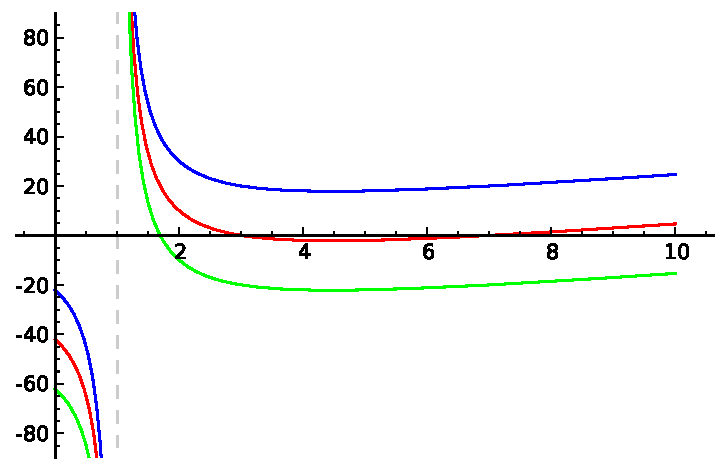
\includegraphics[height=4.5cm]{graphen}
\end{center}\newpage

%%%%%%%%%%%%%%%%%%%%%%%%%%%%%%%%%%%%%%
\subsection{Symbolisches Rechnen}
%%%%%%%%%%%%%%%%%%%%%%%%%%%%%%%%%%%%%%

Wir wollen uns nun ein wenig mit symbolischem Rechnen vertraut machen; dazu zählt das numerische Lösen von Integralen, 
sicherlich aber auch die Vereinfachung oder die Faktorisierung eines Terms. Wir betrachten einige Beispiele:\newline
Wir möchten gerne das Integral $\int_0^\infty x^4 e^{-x} dx$ numerisch berechnen, dazu benötigen wir lediglich
\begin{sagein}
integrate(x^4*exp(-x),x,0,oo)
\end{sagein}
und erhalten als Ausgabe 
\begin{sage}
  24
\end{sage}.
Wollen wir eine Stammfunktion von $\frac{1+\sin (x)}{1+\cos(x)}$ berechnen, so genügt uns die Deklaration zweier Funktion f
und g wie folgt:
\begin{sagein}
f(x) = (1+sin(x))/(1+cos(x))
g = f.integrate(x);g
\end{sagein}
\begin{sage}
x |--> sin(x)/(cos(x) + 1) - log(cos(x) + 1)
\end{sage}
Die Funktion g sieht eher unschön aus, wir möchten sie daher vereinfachen und benutzen dafür
\begin{sagein}
g.full_simplify()
\end{sagein}
\begin{sage}
x |--> -((cos(x) + 1)*log(cos(x) + 1) - sin(x))/(cos(x) + 1)
\end{sage}
Die Verschönerung hat hier nur bedingt geklappt, aber der Versuch war es wert und oft erhält man wirklich ein schöneres 
Ergebnis als zuvor. Ein wenig effektiver funktioniert es mit ($\frac{e^x -1}{e^{(1/2)x}+1}$)
\begin{sagein}
g = (exp(x)-1)/(exp(x/2)+1)
g.simplify_radical()
\end{sagein}
\begin{sage}
 e^(1/2*x) - 1
\end{sage}
Es gibt noch andere Möglichkeiten, Termen ein schöneres Aussehen zu geben. Betrachten wir den Term
\begin{sage}
x^4 - 10*x^3 + 35*x^2 - 50*x + 24
\end{sage}
und fragen uns: Können wir ihn Faktorisieren? Eine Antwort darauf liefert 
\begin{sagein}
factor(x^4 - 10*x^3 + 35*x^2 - 50*x + 24)
\end{sagein}
\begin{sage}
(x - 4)*(x - 3)*(x - 2)*(x - 1)
\end{sage}
Als kleine Probe können wir die Faktorisierung rückgängig machen:
\begin{sagein}
expand(_)
\end{sagein}
\begin{sage}
x^4 - 10*x^3 + 35*x^2 - 50*x + 24
\end{sage}
\textbf{Bemerkung:} Wir erinnern uns, dass \_ eine Referenz auf die letzte Ausgabe ist.\newline
Wir können Terme Terme auch bzgl. einer Variablen sortieren lassen:\newline
\begin{sagein}
var('b,a')
g = x^2+2*x+b*x^2+sin(x)+a*x
g.collect(x)
\end{sagein}
\begin{sage}
(b + 1)*x^2 + (a + 2)*x + sin(x)
\end{sage}
Zuletzt steht uns hier noch die Partialbruchzerlegung zur Verfügung:\newline
\begin{sagein}
g = x^ 2/( x^ 2- 1)
g.partial_fraction()
\end{sagein}
\begin{sage}
1/2/(x - 1) - 1/2/(x + 1) + 1
\end{sage}
\newpage

%%%%%%%%%%%%%%%%%%%%%%%%%%%%%%%%%%%%%%
\subsection{Analytische Geometrie und Lineare Algebra}
%%%%%%%%%%%%%%%%%%%%%%%%%%%%%%%%%%%%%%

Wir wollen uns ein wenig mit analytischer Geometrie und linearer Algebra beschäftigen und zu Anfang mal den Schnittpunkt einer Ebene mit einer Geraden 
berechnen. Dazu sei die Ebene E gegeben durch
\[ E: \vec{x}= 
\left ( \begin{array}{c}  2 \\ 1 \\ -1 \end{array} \right) +l 
\left ( \begin{array}{c}  1 \\ -1 \\ -1 \end{array} \right) +m
\left ( \begin{array}{c}  -3 \\ 1 \\ 4 \end{array} \right), \quad l,m
\in \mathbb{R}
\]
und die Gerade g
\[
g: \vec{x}=
\left ( \begin{array}{c}  3 \\ 0 \\ 1 \end{array} \right) +k
\left ( \begin{array}{c}  4 \\ -1 \\ 2 \end{array} \right), \quad k \in \mathbb{R}
\]
Gleichsetzen ergibt: 
\[ 
\left ( \begin{array}{c}  2 \\ 1 \\ -1 \end{array} \right) +l 
\left ( \begin{array}{c}  1 \\ -1 \\ -1 \end{array} \right) +m
\left ( \begin{array}{c}  -3 \\ 1 \\ 4 \end{array} \right) = \left ( \begin{array}{c}  3 \\ 0 \\ 1 \end{array} \right) +k
\left ( \begin{array}{c}  4 \\ -1 \\ 2 \end{array} \right)
\] oder {
\[ 
\underbrace{\left(   
\begin{array} {ccc} 
1 & -3 & -4\\
-1 & 1 & 1 \\
-1 & 4 & -2  
\end{array} \right)}_{\displaystyle =:A} 
\underbrace{\left ( \begin{array}{c}  l \\ m \\ k \end{array}
  \right)}_{\displaystyle =:L} = \underbrace{\left ( \begin{array}{c}  1 \\ -1 \\ 2
  \end{array} \right)}_{\displaystyle =:b}
\] }
oder $A L=b$.
Wir wollen nun lineare Gleichungssysteme (wie dieses) wie gewöhnlich durch MAtrizen beschreiben und via Sage lösen. Dazu benötigen wir ein paar Grundlagen:
\begin{itemize}
\item Definieren der Matrix $A$
\begin{sagein}
A = matrix([[1,-3,-4],[-1,1,1],[-1,4,-2]]); A
\end{sagein}
\begin{sage}
[ 1 -3 -4]
[-1  1  1]
[-1  4 -2]
\end{sage}
\item Definieren des Vektors $b$
\begin{sagein}
b = vector([1,-1,2])
\end{sagein}
\item Lösen von  $A \ L=b$
\begin{sagein}
A.solve_right(b)
\end{sagein}
oder 
\begin{sagein}
A\b
\end{sagein}
ergibt
\begin{sage}
(6/5, 3/5, -2/5)
\end{sage}
\item Einsetzen in die Geradengleichung
\begin{sagein}
x_s = matrix([g1,g2,g3]).subs(k=L[2]); x_s
\end{sagein}
\begin{sage}
[7/5 2/5 1/5]
\end{sage}
\end{itemize}
So haben wir nun recht aufwandsarm den Schnittpunkt der beiden Objekte E und g erhalten. Wir geben noch einen kurzen Ausblick auf weitere 
Matrizenoperationen:\newline
\begin{sagein}
B = matrix([[1,0,0],[0,1,1],[1,1,1]])
A*B; A-B; A+B
\end{sagein}
\begin{sage}
[-3 -7 -7]  [ 0 -3 -4] [ 2 -3 -4]
[ 0  2  2]  [-1  0  0] [-1  2  2]
[-3  2  2]  [-2  3 -3] [ 0  5 -1]
\end{sage}
Berechnen der Inversen (mit Probe)
\begin{sagein}
$A^(-1)$, A*A^(-1)
\end{sagein}
\begin{sage}
[  -2/5 -22/15   1/15]
[  -1/5   -2/5    1/5]
[  -1/5  -1/15  -2/15]

[1 0 0]
[0 1 0]
[0 0 1]
\end{sage}
Wir wollen uns das Ganze mal visualisieren, hierzu bietet uns Sage den 3D plot:
\begin{sagein}
var('l,m'); E1 = 2+l-3*m; E2 = 1-l+m; E3 =-1-l+4*m
p = parametric_plot3d([E1,E2,E3],(l,-2,2),(m,-2,2), color='green', opacity=0.8)
var('k'); g1 = 3+4*k; g2 = -k; g3 = 1+2*k
p += parametric_plot3d( (g1,g2,g3), (k, -3, 3),thickness='3' ) 
p.show()
\end{sagein}
\begin{center}
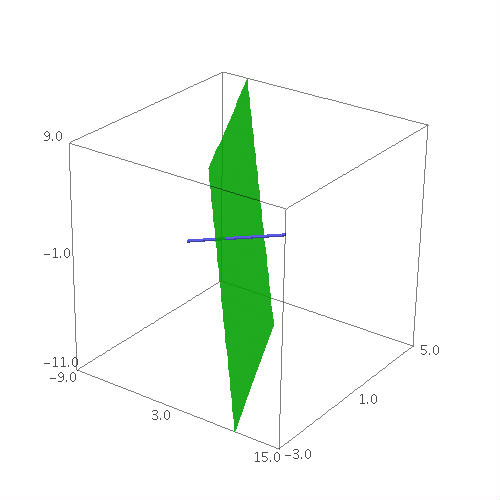
\includegraphics[width=0.7\textwidth]{ebene2}
\end{center}
\textbf{Bemerkung:} In Sage lässt sich der 3D plot drehen.
\newpage

%%%%%%%%%%%%%%%%%%%%%%%%%%%%%%%%%%%%%%
\subsection{Programmieren}
%%%%%%%%%%%%%%%%%%%%%%%%%%%%%%%%%%%%%%

\begin{itemize}
 \item Wir möchten eine einzeilige Funktion definieren. Dies geschieht via
  \begin{sagein}
  def <name>(<Argumente>) : return <Rueckgabe>
  \end{sagein}
  Beispiel: 
  \begin{sagein}
  def fd(ex) : return diff(ex)
  fd(x^2)
  \end{sagein}
  \begin{sage}
  2*x
  \end{sage}
 \item Wir können Objekte in Listen und Tupeln zusammenfassen:\newline
  Eine \emph{Liste} ist in Sage (und Python) mit \isage{[..,..]} gekennzeichnet
  \begin{sagein}
  liste = [21,22,24,23]
  liste.sort(); liste 
  \end{sagein}
  \begin{sage}
  [21, 22, 23, 24]
  \end{sage}
  Ein \emph{Tuple} ist in Sage (und Python) mit \isage{(..,..)} gekennzeichnet 
  \begin{sagein}
  tuple = (liste[0], liste[2])
  tuple, tuple[0]
  \end{sagein}
  \begin{sage}
  ((21, 24), 21) 
  \end{sage}
  Liste von ganzen Zahlen von \isage{a} bis \isage{b}
  \begin{sagein}
  [a..b] ; range(a,b+1)
  \end{sagein}
 \item Es gibt einzeilige (bedingte) Schleifen:
  \begin{sagein}
  [<expr(var)> for <var> in <range|liste>] 
  [<expr(var)> for <var> in <range|liste> if <expr>] 
  \end{sagein}
  Beispiel:
  \begin{sagein}
  [m^2 for m in [1..5] ]
  \end{sagein}
  \begin{sage}
  [1, 4, 9, 16, 25]
  \end{sage}
  Beispiel mit Abfrage:
  \begin{sagein}
  [m^2 for m in [1..5] if m%2==0]
  \end{sagein}
  \begin{sage}
  [4, 16]
  \end{sage}
\end{itemize}

%%%%%%%%%%%%%%%%%%%%%%%%%%%%%%%%%%%%%%
\subsection{Zahlentheorie}
%%%%%%%%%%%%%%%%%%%%%%%%%%%%%%%%%%%%%%

Wir sind nun in der Lage, etwas kompliziertere Aufgabenstellungen zu bearbeiten:\newline
\begin{enumerate}
\item Die Fermatschen Primzahlen sind gegeben durch $F_n=2^{2^n} +1$. Wir wollen die kleinste dieser Zahlen finden, die keine Primzahl ist. Dazu 
schreiben wir uns ein kleines Programm:
\begin{sagein}
def F(n): return 2^(2^n)+1
[[F(m),is_prime(F(m))] for m in range(1,6)]
\end{sagein}
\begin{sage}
[[5, True], [17, True], [257, True], [65537, True], [4294967297, False]]
\end{sage}
Uns interssieren nun noch die Teiler von $F_5$
\begin{sagein}
divisors(int(F(5)))
\end{sagein}
\begin{sage}
[1, 641, 6700417, 4294967297]
\end{sage}
\item Wir möchten eine Liste der Primzahlen bis 100:
\begin{sagein}
menge = range(1,101)
[m for m in menge if is_prime(m)]
oder filter(is_prime,menge)
\end{sagein}
\begin{sage}
[2, 3, 5, 7, 11, 13, 17, 19, 23, 29, 31, 37, 41, 43, 47, 53, 59, 61, 67, 71, 73, 79, 83, 89, 97]
\end{sage}
\item Die Mersenne Primzahlen sind gegeben durch $2^p-1$, dabei $p$ Primzahl. Wir wollen die Mersenne Primzahlen im Bereich $\leq200$ bestimmen:
\begin{sagein}
menge = range(1,201)
primes = [m for m in menge if is_prime(m)]
[2^m-1 for m in primes if is_prime(2^m-1)]
\end{sagein}
\begin{sage}
[3, 7, 31, 127, 8191, 131071, 524287, 2147483647, 2305843009213693951,
618970019642690137449562111, 162259276829213363391578010288127,
170141183460469231731687303715884105727]
\end{sage}
\item Wir wollen für die Zahlen $\leq1000$ bestimmen, wieviele Zahlen 1,2,3,... Teiler haben:
\begin{sagein}
menge = range(1,1001)
liste = [number_of_divisors(int(m)) for m in menge]
[(i,len([m for m in liste if m==i]))for i in range(1,51)]
\end{sagein}

\begin{sage}
[(1, 1), (2, 168), (3, 11), (4, 292), (5, 3), (6, 110), (7, 2), (8,
180), (9, 8), (10, 22), (11, 0), (12, 97), (13, 0), (14, 5), (15, 4),
...
\end{sage}
\end{enumerate}
Bis hierher haben wir einen kleinen Rundumblick genommen, einige sehr elementare Grundlagen kennengelernt und sind schon recht vertraut mit 
Sage. Vieles von dem, was wir bisher gesehen haben, wird uns wieder begegnen, wenn wir uns weiter mit Sage befassen.
%%%%%%%%%%%%%%%%%%%%%%%%%%%%%%%%%%%%%%
\chapter{Grundlagen}
\section{Interna}
%%%%%%%%%%%%%%%%%%%%%%%%%%%%%%%%%%%%%%
Um Sage richtig verstehen zu können, ist es wichtig, das ``Innenleben'' zu kennen- hierzu wollen wir uns anschauen, welche Datentypen Sage 
kennt und wie es mit ihnen umgeht. Dazu stellen wir uns unter Anderem folgende Fragen:\newline
Betrachte:
\begin{sagein}
f = x^2-3*x-18
\end{sagein}
\begin{itemize}
\item Wie geht Sage mit der Unbekannten $x$ um?
\item Welchen Datentyp hat $f$?
\item Was kann ich mit $f$ machen?
\end{itemize}
\begin{enumerate}
  \item \textbf{Bezeichner:}
    \begin{itemize}
    \item \emph{Bezeichner} sind Namen, wie z.B. $x$ oder $f$. Sie können
    im mathematischen Kontext sowohl Variablen als auch Unbestimmte repräsentieren.
    \item Bezeichner sind aus Buchstaben, Ziffern und
    Unterstrich \_ zusammengesetzt.
    \item Sage unterscheidet zwischen Groß- und Kleinschreibung.
    \item Bezeichner dürfen nicht mit einer Ziffer beginnen
    \begin{itemize}
    \item zulässige Bezeichner:\isage{x}, \isage{f}, \isage{x23}, \isage{_x_1}
    \item unzulässige Bezeichner:\isage{12x}, \isage{p~}, \isage{x>y}, \isage{Das System}
    \end{itemize}
  \end{itemize}
  \item\textbf{Wert eines Bezeichners:}
    \begin{itemize}
    \item Der \emph{Wert} eines Bezeichners  ist ein \emph{Objekt} eines bestimmten
    \emph{Datentyps}.
    \item Ein \emph{Datentyp} ist durch seine Eigenschaften gegeben. \\
    \textbf{Beispiel}: Natürliche Zahlen, rationale Zahlen, Bezeichner, Zeichenketten, \ldots  
    \item Ein \emph{Objekt} ist eine Instanz (Einheit) eines Datentyps.
    \end{itemize}
  \item \textbf{Zuweisungsoperator = :}
    \begin{itemize}
    \item {\color{blue} \isage{bez=wert}}: Zuweisung des Wertes \isage{wert} zu dem Bezeichner \isage{bez}.
    \item {\color{blue} \isage{func(arg)=expr(arg)}}: Definition der Funktion \isage{func} mit dem Argument \isage{arg} und Zuweisung des Ausdrucks \isage{expr} zu (abhängig von \isage{arg})
    %\item Rückgabeparameter ist die rechte Seite (Eine Ausgabe erfolgt jedoch normalerweise nicht)
    \item \textbf{Warnung:} Wir unterscheiden stets zwischen dem Zuweisungsoperator {\color{blue} $=$} und
    dem logischen Operator {\color{blue} $==$}.   
    \item {\color{blue} \isage{reset('bezeichner')}}: Löschen von Zuweisungen/Variablen.\newline
    \item\textbf{Beispiele:}
      \begin{sagein}
      N=6; N
      \end{sagein}
      \begin{sage}
	6
      \end{sage}
      \begin{sagein}
      x,y = var('x,y'); f = x+2*x*x-y; g(x) = x^2; f,g
      \end{sagein}
      \begin{sage}
      (2*x^2 + x - y, x |--> x^2)
      \end{sage}
      \begin{sagein}
      x=pi;y = cos(x); x,y
      \end{sagein}
      \begin{sage}
	(pi, -1)
      \end{sage}
  \item \textbf{Auswertung:}
    \begin{itemize}
    \item Der \emph{Bezeichner} ist der Name einer Unbekannten.
    \item Die \emph{Auswertung} eines Bezeichners erfolgt ohne die Benutzung von bekannten Zuweisungen.
    \item Der \emph{Wert} bezeichnet die Auswertung zum Zeitpunkt der Zuweisung.
    \item \textbf{Beispiele}
    \begin{sagein}
    var('a') ; f(x) = x*x-3*x-a
    \end{sagein}
    \begin{sage}
    x |--> x^2 - a - 3*x
    \end{sage}
    \begin{sagein}
    f(a=2)
    \end{sagein}
    \begin{sage}
    x^2 - 3*x - 2 
    \end{sage}
    \begin{sagein}
    f(1)
    \end{sagein}
    \begin{sage}
      -a - 2
    \end{sage}
    \begin{sagein}
    f(1,a=2)
    \end{sagein}
    \begin{sage}
      -4
    \end{sage}
    \end{itemize}
  \end{itemize}
  \item\textbf{Datentypen:}
    \begin{center}
      \begin{tabular}{|lll|}
      \hline
      Typ & Bedeutung & Beispiel\\
      \hline
      \isage{integer} & ganze Zahlen & \isage{-3,0,100}\\
      \isage{rational} & rationale Zahlen & \isage{7/11}\\
      \isage{float} & Gleitpunktzahl & \isage{0.123}\\
      \isage{complex} & komplexe Zahlen & \isage{complex(1,3)}\\
      \isage{expression} & symbolische Ausdrücke & \isage{x+y} \\
      \isage{bool} & logische Werte: true/false& \isage{bool(1<2)} \\
      \hline
      \end{tabular}
    \end{center}
    \textbf{Beispiele:}\newline
    \begin{sagein}
    type(5)
    \end{sagein}
    \begin{sage}
      <type 'sage.rings.integer.Integer'>
    \end{sage}
    \begin{sagein}
    f = x^2-3*x-18; type(f)
    \end{sagein}
    \begin{sage}
      <type 'sage.symbolic.expression.Expression'>
    \end{sage}
    \begin{sagein}
    type(x)
    \end{sagein}
    \begin{sage}
      <type 'sage.symbolic.expression.Expression'>
    \end{sage}
    \begin{sagein}
    f+f
    \end{sagein}
    \begin{sage}
    2*x^2 - 6*x - 36
    \end{sage}
  \item\textbf{Operatoren:} 
    \begin{itemize}
    \item Typische \emph{Operatoren} sind \verb~+,-,*,/,..~
    \item In Sage werden Objekte immer durch Funktionen miteinander
    verbunden. Operatoren sind äquivalent zu Funktionen.
    %\item Operatoren sind in Sage auch als Funktionen realisiert.
    %\item Für wichtige Operatoren gibt es die gewohnte
    %Kurzschreibweise.
    \item Kombination verschiedener Operatoren: Die Regeln der \emph{Bindungsstärke} gelten (Punktrechnung vor Strichrechnung); Die Ordnung kann
    durch Klammersetzung geändert werden.
    \item Wichtige mathematische Operatoren:
      \begin{center}
      \begin{tabular}{|c|l|}
      \hline
      Operator/Funktion &  Erklärung\\
      \hline
      \hline
      \verb!+! & Addition \\
      \verb!-! & Subtraktion\\
      \verb!*! & Multiplikation \\
      \verb!/! & Division\\
      \verb!^! & Potenz\\
      \verb!%! &  Rest bei Division\\
      \verb!factorial()! & Fakultät \\
      \hline
      \end{tabular}
      \end{center}
     \end{itemize}
  \item\textbf{Ausdrücke:}
    \begin{itemize}
    \item Bausteine von Ausdrücken heißen \emph{Operanden}.
    \item {\color{blue} \isage{Ausdruck.nops()}}: Anzahl der Operanden. 
    \item {\color{blue} \isage{Ausdruck.operands()}}: Operanden selbst. 
    \item {\color{blue} \isage{Ausdruck.has(a)}}: Untersuchung ob $a$ ein Operand von \isage{Ausdruck} ist.
    \item Die Befehle beziehen sich jeweils auf die automatisch vereinfachten Objekte.\newpage
    \item \textbf{Beispiele:}
      \begin{sagein}
      _=var('z,y');f = x*z+3*x+sqrt(y)
      f.operands(),(f.operands())[1],((f.operands())[1]).nops()
      \end{sagein}
      \begin{sage}
      ([x*z, 3*x, sqrt(y)], 3*x, 2)
      \end{sage}
      \begin{sagein}
      f.has(z), f.has(6) 
      \end{sagein}

      \begin{sage}
      (True, False)
      \end{sage}
  \end{itemize}
  \item\textbf{Automatische Vereinfachung:}
    Sage führt oft automatische Vereinfachungen durch. Ansonsten muß
    der Benutzer gezielt Vereinfachungen anfordern.
    \begin{sagein}
    sin(15*pi), exp(0)
    \end{sagein}
    \begin{sage}
      (0, 1)
    \end{sage}
    \begin{sagein}
    2*Infinity-5
    \end{sagein}
    \begin{sage}
      +Infinity
    \end{sage}
    \begin{sagein}
    y = (-4*x+x^2+4)*(7*x+x^2+12); y
    \end{sagein}
    \begin{sage}
    (x^2 - 4*x + 4)*(x^2 + 7*x + 12)
    \end{sage}
    \begin{sagein}
    y.full_simplify()
    \end{sagein}
    \begin{sage}
    x^4 + 3*x^3 - 12*x^2 - 20*x + 48
    \end{sage}
  \item\textbf{Ausgabe von Variablen in Texten:}
    \begin{sagein}
    print "Text %<format> und %<format> ... " % (x,y,...)}
    \end{sagein}
    \begin{itemize}
    \item \isage{<format>} kann z.B. \isage{i} für \isage{integer} oder \isage{f} für \isage{float} sein
    \item Es kann beliebig viele format-Platzhalter geben
    \end{itemize}
    Beispiele: 
    \begin{sagein}
    x = 4;y = 6
    print "x ist %i und y ist %i" % (x,y)
    \end{sagein}
    \begin{sage}
    x ist 4 und y ist 6
    \end{sage}
    \begin{sagein}
    x = [var("x%i" % k) for k in [1..3]]; x
    \end{sagein}
    \begin{sage}
    [x1, x2, x3]
    \end{sage}
\end{enumerate}
%%%%%%%%%%%%%%%%%%%%%%%%%%%%%%%%%%%%%%
\section{Praxisbezug}
%%%%%%%%%%%%%%%%%%%%%%%%%%%%%%%%%%%%%%
Wir kommen nun zurück zu einigen praktischen Anwendungen des eben neu Gelernten- einiges Altbekannte wird uns wiederbegegnen:
%%%%%%%%%%%%%%%%%%%%%%%%%%%%%%%%%%%%%%
\subsection{Dictionaries}
%%%%%%%%%%%%%%%%%%%%%%%%%%%%%%%%%%%%%%
\begin{itemize}
\item Dictionaries bestehen aus \emph{Assoziationen} der Form \verb+<Index>:<Wert>+. 
\item Definition:
\begin{sagein}
d = {<Index1>:<Wert1>,<Index2>:<Wert2>,...}
\end{sagein}
\item Zugriff:
\begin{sagein}
d[<Index>]
\end{sagein}
\item \textbf{Beispiel:}
\begin{sagein}
var('x,y,z');d = {x:21,y:5,z:42==y}
d[x],d[z],d[z].rhs()
\end{sagein}
\begin{sage}
(21, 42 == y, y)
\end{sage}
\end{itemize}
%%%%%%%%%%%%%%%%%%%%%%%%%%%%%%%%%%%%%%
\subsection{Funktionen und Abfragen}
%%%%%%%%%%%%%%%%%%%%%%%%%%%%%%%%%%%%%%
\begin{itemize}
\item Anonyme Funktionen sind Funktionen die keinen aufrufbaren Namen besitzen (Sie sind ein Funktionen-Objekt)
\item Dies ist sinnvoll innerhalb von Konstrukten oder Aufrüfen anderer Funktionen.
\item Syntax:
\begin{sagein}
lambda <parameter_list>: <expression> 
\end{sagein}
\item \textbf{Beispiel}
\begin{sagein}
menge = [1,2,3,4,5]
map(lambda x: x^2,menge)
\end{sagein}
\begin{sage}
 [1, 4, 9, 16, 25]
\end{sage}
\item Objekte besitzen Funktionen, sogenannte \emph{Objekt-Methoden}. 
\item Ein Objekt kennt alle auf sich selbst anwendbaren Funktionen; Nur einige Methoden sind als globale Funktionen benutzbar (wie z.B. \isage{map()})\newpage
\item Beispiel
 \begin{sagein}
f = 1 +x -x^2; f.operands(); operands(f)
\end{sagein}
\begin{sage}
[-x^2, x, 1]
Traceback (click to the left of this block for traceback)
...
NameError: name 'operands' is not defined
\end{sage}
\textbf{Bemerkung:}\newline
 f.operands() erzeugt die erste Zeile.\newline
 Den ErrorCode verursacht operands(f).
\item Bereits bekannte Schleifen: \verb+[.. for .. in ..]+-Konstrukt. Die \verb+for+-Schleife kann  auch
ganze Blöcke wiederholen.
\begin{sagein}
for <indexvar> in <expr>/<list>:
    <Code-Block>
else:
    <Code-Block>
\end{sagein}
\textbf{Beispiel:}
\begin{sagein}
x = 2; y = 2
for k in [1..4]:
    x = x +k
    y = y^k
x,y
\end{sagein}
\begin{sage}
(12, 16777216)
\end{sage}
\textbf{Wichtig:} In Python/Sage ist solch ein Code-Block dadurch gekennzeichnet, dass er mit einem \textbf{:} eingeleitet wird und um ein TAB eingerückt ist!
\item Einfache Abfragen werden mittels \isage{if/else} realisiert. Diese können für ganze Blöcke genutzt werden:
\begin{sagein}
if <boolean expr>:
    <Code-Block>
\end{sagein}
\textbf{Beispiel:}
\begin{sagein}
x = 3; y = 2
if x > y :
    z = x
else:
    z = y
z
\end{sagein}
\begin{sage}
3
\end{sage}
\end{itemize}
%%%%%%%%%%%%%%%%%%%%%%%%%%%%%%%%%%%%%%
\subsection{Ausdrücke}
%%%%%%%%%%%%%%%%%%%%%%%%%%%%%%%%%%%%%%
%\begin{itemize}
    Ausdrücke können beliebig addiert, subtrahiert, multipliziert und
    dividiert werden.\\ 
    \textbf{Beispiel:}
    \begin{itemize}
    \item Definition
    \begin{sagein}
    var('x,y'); f = x*x+3*x+y; g = x-y
    \end{sagein}
    \item Potenz
    \begin{sagein}
    f^g
    \end{sagein}
    \begin{sage}
    (x^2 + 3*x + y)^(x - y)
    \end{sage}
    \item Addition / Subtraktion
    \begin{sagein}
    f+g, f-g
    \end{sagein}
    \begin{sage}
    (x^2 + 4*x, x^2 + 2*x + 2*y)
    \end{sage}
    \item Multiplikation/ Division
    \begin{sagein}
    f*g, f/g
    \end{sagein}
    \begin{sage}
    ((x - y)*(x^2 + 3*x + y), (x^2 + 3*x + y)/(x - y))
    \end{sage}
    \end{itemize}
    {\color{blue} \isage{a.collect(<unknown>)}}: der Ausdruck \isage{a} wird bzgl. der \isage{unknown} Variablen sortiert.\\
    \textbf{Beispiel:}
    \begin{sagein}
    f = a*x^2+a*x+x^3+sin(x)+b*x+4*x+x*sin(x)
    f.collect(x)
    \end{sagein}
    \begin{sage}
    a*x^2 + x^3 + (a + b + sin(x) + 4)*x + sin(x)
    \end{sage}
    \begin{sagein}
    f.collect(x*sin(x))
    \end{sagein}
    \begin{sage}
    a*x^2 + x^3 + a*x + b*x + x*sin(x) + 4*x + sin(x)
    \end{sage} 
    {\color{blue} \isage{a.combine()}}:  der Ausdruck wird durch die Potenzgesetze zusammengefaßt.\\
    \textbf{Beispiel:}
    \begin{sagein}
    g = x^(a)*x^(b)
    g.combine()
    \end{sagein}
    \begin{sage}
    x^(a + b)
    \end{sage}
    {\color{blue} \isage{a.expand()}}: Ausmultiplizieren.\\
    {\color{blue} \isage{a.expand_trig()}}: Ausmultiplizieren mit Nutzung der trigonometrischen Eigenschaften.\newpage
    \textbf{Beispiel:}
    \begin{sagein}
    expand((x+2)^4)
    \end{sagein}
    \begin{sage}
    x^4 + 8*x^3 + 24*x^2 + 32*x + 16
    \end{sage}
    \begin{sagein}
    (sin(x+y)).expand_trig()
    \end{sagein}
    \begin{sage}
    sin(x)*cos(y) + sin(y)*cos(x)
    \end{sage}
    \begin{sagein}
    a = (16*x-13)^2 == (3*x+5)^2/2
    a.expand()
    \end{sagein}
    \begin{sage}
    256*x^2 - 416*x + 169 == 9/2*x^2 + 15*x + 25/2
    \end{sage}
    \begin{sagein}
    a.expand('left')
    \end{sagein}
    \begin{sage}
    256*x^2 - 416*x + 169 == 1/2*(3*x + 5)^2
    \end{sage}
    \begin{sagein}
    a.expand('right')
    \end{sagein}
    \begin{sage}
    (16*x - 13)^2 == 9/2*x^2 + 15*x + 25/2
    \end{sage}
    {\color{blue} \isage{factor(Ausdruck)}}:  Faktorisieren von Ausdrücken. 
    \begin{itemize}
    \item Sage faktorisiert nur, wenn die resultierenden Koeffizienten rationale 
    Zahlen sind. 
    \item Bei rationalen Funktionen wird ein gemeinsamer Hauptnenner gesucht.
    \end{itemize}
    \textbf{Beispiel:}
    \begin{sagein}
    factor(x^2-2), factor(x^2-9/4)
    \end{sagein}
    \begin{sage}
    (x^2 - 2, 1/4*(2*x - 3)*(2*x + 3))
    \end{sage}
    \begin{sagein}
    factor(2 - 2/(x^2-1))
    \end{sagein}
    \begin{sage}
    2*(x^2 - 2)/((x - 1)*(x + 1))
    \end{sage}
    {\color{blue} \isage{f.partial_fraction()}}: Zerlegung eines rationalen Ausdruck $f$ in eine
    Summe rationaler Terme (Zählergrad $<$ Nennergrad) (Partialbruchzerlegung).\\
    \textbf{Beispiel:}
    \begin{sagein}
    f = x^2/(x^2-1); f.partial_fraction()
    \end{sagein}
    \begin{sage}
    1/2/(x - 1) - 1/2/(x + 1) + 1
    \end{sage}
    \begin{sagein}
    f = (x^2+2*x+3)/(x^3+4*x^2+5*x+2); f 
    \end{sagein}
    \begin{sage}
    (x^2 + 2*x + 3)/(x^3 + 4*x^2 + 5*x + 2)
    \end{sage}
    {\color{blue} \isage{f.simplify()}}: simple Vereinfachung (Potenzen).
    {\color{blue} \isage{f.simplify_<target>()}}: vereinfacht den Ausdruck $f$ mit der Methode \isage{<target>}. Mögliche targets sind
    \begin{itemize}
    \item \isage{trig}: trigonometrisch
    \item \isage{rational}: rational
    \item \isage{radical}: log/ln/exp
    \item \isage{factorial}: Nutzung der Fakultät
    \item \isage{full}: alle Vereinfachungen
    \end{itemize}
    \textbf{Beispiele:}
    \begin{sagein}
    (2 - 2/(x^2-1)).simplify_rational()
    \end{sagein}
    \begin{sage}
    2*(x^2 - 2)/(x^2 - 1)
    \end{sage}
     \begin{sagein}
	  f = x/(x+y)+y/(x+y)-sin(x)^2-cos(x)^2
	  f.simplify_rational()
	  \end{sagein}
	  \begin{sage}
	  -sin(x)^2 - cos(x)^2 + 1
	  \end{sage}
     \begin{sagein}
	  g = sqrt(997)-(997^3)^(1/6)
	  g.simplify()
	  \end{sagein}
	  \begin{sage}
	  0
	  \end{sage}
    \begin{sagein}
	(tan(x)).simplify_trig()
	\end{sagein}
	\begin{sage}
	sin(x)/cos(x)
	\end{sage}
    \begin{sagein}
	a = (2^(1/3)+4^(1/3))^3-6*(2^(1/3) + 4^(1/3))-6
	a.simplify_full() 
	\end{sagein}
	\begin{sage}
	0
	\end{sage} 
%%%%%%%%%%%%%%%%%%%%%%%%%%%%%%%%%%%%%%
\subsection{Gleichungen, Vergleiche, Logik}
%%%%%%%%%%%%%%%%%%%%%%%%%%%%%%%%%%%%%%
GLEICHUNGEN
    \begin{itemize}
	\item lineares Beispiel
	\begin{sagein}
	var('x,y')
	Gleichungen = [x+y == 1, x-y == 1]
	solve(Gleichungen,x,y)
	\end{sagein}
	\begin{sage}
	  [[x == 1, y == 0]]
	\end{sage}
	\item nichtlineares Beispiel
	\begin{sagein}
	Gleichungen1 = [x+y == 1,(x-y)^2 == 1]
	solve(Gleichungen1,x,y)
	\end{sagein}
	\begin{sage}
	  [[x == 0, y == 1], [x == 1, y == 0]]
	\end{sage}
	\end{itemize}
VERGLEICHE
        \begin{itemize}
	\item Operator {\color{blue} \isage{==}}: Überprüfung zweier Objekte auf Gleichheit.\\
	\isage{a==b} ist wahr (richtig), wenn $a$ und $b$ die gleichen Auswertungen
	besitzen (und vom gleichen Typ sind). 
	\item {\color{blue} \isage{bool(Ausdruck)}}: Überprüfung von Aussagen. Ergebnis: \isage{True} oder
	\isage{False}.
	\item Operator {\color{blue} \isage{<>}}:  Überprüfung zweier Objekte auf Ungleichheit. \\
	\isage{a<>b} ist \isage{True}, falls $a$ nicht gleich $b$
	ist. 
	\end{itemize}
        \textbf{Beispiele:}
	   \begin{sagein}
		bool(4-3==1)
		\end{sagein}
		\begin{sage}
		  True
		\end{sage}
	   \begin{sagein}
		bool(4*x==x); x=0; bool(4*x==x)
		\end{sagein}
		\begin{sage}
		False
		True
		\end{sage}
	    \begin{sagein}
		bool(x==0); bool(x<>0)
		\end{sagein}
		\begin{sage}
		True
		False
		\end{sage}
	   \begin{sagein}
		bool(0.5==1/2)
		\end{sagein}
		\begin{sage}
		  True
		\end{sage}
	   \begin{sagein}
		type(0.5); type(1/2)
		\end{sagein}
		\begin{sage}
		<type 'sage.rings.real_mpfr.RealLiteral'>
		<type 'sage.rings.rational.Rational'>
		\end{sage}
LOGIK
\begin{itemize}
 \item  Logisches 'und' (\isage{and})
\item Logisches 'oder' (\isage{or}) 
\item Logisches 'nicht' (\isage{not})
\end{itemize}
\textbf{Beispiel:}
\begin{sagein}
true and false, true or false, not true
\end{sagein}
\begin{sage}
 (False, True, False)
\end{sage}
\begin{itemize}
 \item Logiktabelle:
\end{itemize}
\begin{center}
\begin{tabular}{|c||c|c|}
\hline
\textbf{and} & \isage{True} & \isage{False}  \\\hline\hline
\isage{True} & \isage{True} & \isage{False}  \\\hline
\isage{False} & \isage{False} & \isage{False} \\\hline
\end{tabular}
\bigskip

\begin{tabular}{|c||c|c|}
\hline
\textbf{or} & \isage{True} & \isage{False} \\\hline\hline
\isage{True} & \isage{True} & \isage{True}  \\\hline
\isage{False} & \isage{True} & \isage{False}  \\\hline
\end{tabular}
\end{center}

GLS

\begin{itemize}
\item {\color{blue}\isage{<gleichungen>}}: System von Gleichungen.
\item  {\color{blue}\isage{<variablen>}}: Danach wird aufgelöst.
\item {\color{blue}\isage{<optionen>}}:
\begin{itemize}
\item {\color{blue}\isage{multiplicities=True}}:  Vielfachheit der Lösungen wird mit ausgegeben.
\item {\color{blue}\isage{solution_dict=True}}: Lösung wird als Dictonary zurück gegeben.
\end{itemize}
\item Bei einzelnen Gleichungen wird der Lösungswert
zurückgegeben. Bei mehreren Gleichungen wird ein System äquivalenter
Gleichungen zurückgegeben.
\end{itemize}
\textbf{Beispiele:}
\begin{sagein}
solve(x^2+x == y/4,x)
\end{sagein}
\begin{sage}
[x == -1/2*sqrt(y + 1) - 1/2, x == 1/2*sqrt(y + 1) - 1/2]
\end{sage}
\begin{sagein}
f = (x-1)^5*(x^2+1)
solve(f == 0, x)
\end{sagein}
\begin{sage}
[x == -I, x == I, x == 1]
\end{sage}
\begin{sagein}
solve(f == 0, x, multiplicities=True)
\end{sagein}
\begin{sage}
([x == -I, x == I, x == 1], [1, 1, 5])
\end{sage}
\begin{sagein}
assume(x>0); solve(x^2+x == y/4,x)
\end{sagein}
\begin{sage}
 [y == 4*x^2 + 4*x]
\end{sage}
\begin{sagein}
solve([x^2-y^2 == 0],[x,y])
\end{sagein}
\begin{sage}
([x == -y, x == y], [1, 1])
\end{sage}
\begin{sagein}
solve([x^2-y^2 == 0, x+y == 1],x,y)
\end{sagein}
\begin{sage}   
[[x == (1/2), y == (1/2)]]
\end{sage}
\begin{sagein}
sol = solve([x^2-y^2 == 0, x+y == 1],x,y, solution_dict=True); sol 
\end{sagein}
\begin{sage}
 [{y: 1/2, x: 1/2}]
\end{sage}
\begin{sagein}
 sol[0][x], sol[0][y]
\end{sagein}
\begin{sage}
 (1/2, 1/2)
\end{sage}
GLS numerisch 
\begin{sagein}
f.find_root(a,b) 
\end{sagein}
Finden von Nullstellen der Gleichung $f$ im Intervall $[a,b]$.\\
\textbf{Beispiel:}
\begin{sagein}
 (x == sin(x)).find_root(-2,2)
\end{sagein}
\begin{sage}
0.0
\end{sage}
%%%%%%%%%%%%%%%%%%%%%%%%%%%%%%%%%%%%%%
\chapter{Mengen und Zahlen}
\section{Mengen}
%%%%%%%%%%%%%%%%%%%%%%%%%%%%%%%%%%%%%%
\begin{quote}
Unter einer \emph{Menge} verstehen wir jede Zusammenfassung $M$ von bestimmten wohlunterschiedenen Objekten $m$ unserer Anschauung oder unseres Denkens zu einem Ganzen.\\
{\tiny (G. Cantor; Beiträge zur Begründung der transfiniten Mengenlehre; Mathematische Annalen; Bd. 46; 1895; S. 481-512) }
\end{quote}
 \begin{itemize}
\item \emph{Element}: Ein Objekt $x$ in der Menge $M$ (\emph{$x \in  M$}). 
\item \emph{Enthalten}: Es gilt für alle $x \in M$ auch $x \in N$ (\emph{$M \subset N$}).
\item \emph{Gleichheit}: Es gilt $M\subset N$ und $N \subset M$ (\emph{$M=N$}).
\end{itemize}

Mengen in Sage:
\begin{sagein}
Set([<element1>,<element2>,...])
\end{sagein}
\begin{itemize}
\item Es ist eine {\color{blue} ungeordnete} Menge von beliebigen
  Objekten. 
\item Mengen in Sage haben den Typ \emph{\isage{set}}.
\item Leere Mengen: \isage{leere_menge = Set([])}. 
\item Zugriff: \isage{M[n]} (Menge $M$, $n\ge0$)
\item Intervallzugriff: \isage{M[i:j]}.
\end{itemize}
Beispiele:
\begin{sagein}
M1 = Set([x, 2,3,pi,sqrt(2)]); M1
\end{sagein}
\begin{sage}
{pi, 2, 3, sqrt(2), x}
\end{sage}
\begin{sagein}
var('y');M2 = Set([y,1,Set([1,y]),2,x]); M2
\end{sagein}
\begin{sage}
{1, y, 2, x, {1, y}}
\end{sage}
Operationen mit Mengen:
\begin{itemize}
\item Anzahl der Elemente in einer Menge:
\begin{sagein}
M1.cardinality()
\end{sagein}
\begin{sage}
  5
\end{sage}
\item Zugriff:
\begin{sagein}
M2[1]; M2[1:4]
\end{sagein}
\begin{sage}
y
[y, 2, x]
\end{sage}
%\item Ändern von Einträgen mit \isage{op} und \isage{subsop} ohne Nebeneffekt:
%\begin{sagein}
%op(M2,3), subsop(M2,3=neu)
%\end{sagein}
%\begin{sage}
%  {1, y}, {1, 2, neu, x, y}
%\end{sage}
\end{itemize}
\begin{itemize}
\item Vereinigung, Differenz, Schnitt:
\begin{sagein}
L1 = Set([1,2,3,a,b]); L2 = Set([a,b,c,4,5])
L1.union(L2), L1.difference(L2), L1.intersection(L2)
\end{sagein}
\begin{sage}
({1, 2, 3, 4, a, c, b, 5}, {1, 2, 3}, {b, a})
\end{sage}
\item Prüfen, ob  ein Element enthalten ist:
\begin{sagein}
a in L1, c in L1
\end{sagein}
\begin{sage}
(True, False)
\end{sage}
\begin{sagein}
Set([1,y]) in M2
\end{sagein}
\begin{sage}
True
\end{sage}
\end{itemize}

\begin{itemize}
\item Auswählen von Elementen mit bestimmten Eigenschaften
\begin{sagein}
M = Set(range(1,15))
filter(is_prime,M)
\end{sagein}
\begin{sage}
  [2, 3, 5, 7, 11, 13]
\end{sage}
\item Erzeugen der Potenzmenge
\begin{sagein}
list(powerset([1,2,3]))
[s for s in Set([1..3]).subsets()]
\end{sagein}
\begin{sage}
[[], [1], [2], [1, 2], [3], [1, 3], [2, 3], [1, 2, 3]]
[{}, {1}, {2}, {3}, {1, 2}, {1, 3}, {2, 3}, {1, 2, 3}]
\end{sage}
\end{itemize}

Ein Filter erzeugt eine Teilmenge aus einer größeren Menge.
\begin{sagein}
M1 = filter(<f>,<M>)
\end{sagein}
\begin{itemize}
\item \isage{f(x)} ist eine Abbildung auf die Boolschen Werte \isage{True/False}. 
\item \isage{M1} ist die Teilmenge  die aus den Elementen $x\in M$ besteht, für die \isage{f(x)} eine wahre Aussage
ergibt. 
\end{itemize}

Beispiel Filter:
\begin{sagein}
M = Set(range(1,101))
def f(x): return bool(mod(x,2)==0)
M2 = Set(filter(f,M))
def f(x): return bool(mod(x,15)==0)
M15 = Set(filter(f,M))
M2.intersection(M15)
\end{sagein} 
\begin{sage}
 {90, 60, 30}
\end{sage}
Alternative:
\begin{sagein}
M2 = Set([m for m in M if mod(m,2)==0])
M15 = Set([m for m in M if mod(m,15)==0])
\end{sagein
Ist Menge \isage{A1} eine Teilmenge von Menge \isage{A}?
\begin{sagein}
A = Set(range(1,11))
A1 = Set(range(1,3))
A2 = Set(range(9,12))
\end{sagein}
\begin{sagein}
A.intersection(A1) == A1
\end{sagein}
\begin{sage}
  True
\end{sage}
\begin{sagein}
A.intersection(A2) == A2
\end{sagein}
\begin{sage}
  False
\end{sage}

%%%%%%%%%%%%%%%%%%%%%%%%%%%%%%%%%%%%%%
\section{Zahlen}
%%%%%%%%%%%%%%%%%%%%%%%%%%%%%%%%%%%%%%
% andere einfuehrung!
Natürliche Zahlen $\mathbb{N} := \{0,1,2,3,\dots\}$:
\begin{enumerate}
\item $0 \in \mathbb{N}$
\item Es gibt eine Nachfolgerabbildung $nf : \mathbb{N} \
  \rightarrow \mathbb{N} \smallsetminus \{ 0 \}$
\item $nf$ ist injektiv.
\item Ist $M \subset \mathbb{N}$ mit $0 \in M$ und folgt für alle  $m \in M$ das
  $nf(m) \in M$ gilt, so ist $M=\mathbb{N}$.
\end{enumerate}
Bemerkungen:
\begin{itemize}
\item Nachfolgefunktion: $nf(m)=m+1$
\item Es besteht ein enger Zusammenhang zwischen den natürlichen
  Zahlen und vollständiger  Induktion.
%TODO:erklaerung  .
\item Sage: kein eigener Datentyp (aber: ganze Zahlen (Integer)). 
\end{itemize}
Sei $M$ eine Menge. Eine {\color{red} Äquivalenzrelation} $R$ auf $M$ ist eine Teilmenge
\[R\subseteq M \times M\]
 mit den folgenden Eigenschaften (Schreibweise: $(x,y) \in R$, $x \sim_R y$, $x \sim y$):
\begin{enumerate}
\item \textbf{Reflexivität:} für alle $x \in M$ gilt $x \sim x$. 
\item \textbf{Symmetrie:} für alle $x,y \in M$ folgt aus $x \sim y$ das $y \sim x$.
\item \textbf{Transitivität:} für alle $x,y,z \in M$ und $x \sim y$, $y \sim z$ folgt
  $x \sim z$.  
\end{enumerate}
\begin{itemize}
\item Sei $\sim_R$ eine Äquivalenzrelation auf einer Menge $M$.
\item Eine Teilmenge $A \subset M$ heißt {\color{red} Äquivalenzklasse}, falls gilt:
\begin{itemize}
\item [(a)] $A \neq \emptyset$.
\item [(b)] $x,y \in A \ \Rightarrow \ x \sim y$.
\item [(c)] $x \in A$, $y \in M$, $x \sim y$ $\Rightarrow$ $y \in A$.
\end{itemize}
\item Eine Äquivalenzrelation zerlegt eine Menge in disjunkte
Äquivalenzklassen.  
\item Andersrum definiert eine disjunkte Zerlegung einer Menge eine Äquivalenzrelation.
\item  Ein $a \in A$ ist ein {\color{red} Repräsentant} der Äquivalenzklasse
$A$. Man schreibt auch $\overline{a}$ oder $a \bmod R$ für ein Äquivalenzklasse $A$. 
\end{itemize}
Ganze Zahlen: $\mathbb{Z}:=\{ 0,1,-1,2,-2,\dots \}$
% das kann abe rbesser...
\begin{itemize}
\item Äquivalenzrelation auf $\mathbb{N} \times \mathbb{N}$:\\
$(m,n) \sim (p,q) \mbox{ genau dann, wenn } m+q=n+p \mbox{ gilt.} $
\item Nichtnegative Zahlen: $(m,0)$. Sie sind paarweise nicht äquivalent
zueinander.
\item Negative Zahlen: $(0,m)$. 
\item Die ganzen Zahlen $\mathbb{Z}$ sind  gegeben durch die Menge
der Äquivalenzklassen.
\item Addition:
\[
\overline{(m,n)}+\overline{(u,v)}:=\overline{(m+u,n+v)}\]
\item Multiplikation:
\[
\overline{(m,n)}\cdot\overline{(u,v)}:=\overline{(m u+nv,mv+nu)}
\]
\end{itemize}
Datentyp \isage{Integer}. \\
\textbf{Beispiele:}
\begin{sagein}
type(5), type(0), type(-5)
\end{sagein}
\begin{sage}
(<type 'sage.rings.integer.Integer'>, 
<type 'sage.rings.integer.Integer'>, 
<type 'sage.rings.integer.Integer'>)
\end{sage}
Division
\begin{sagein}
type(5*4), type(5/4)
\end{sagein}
\begin{sage}
(<type 'sage.rings.integer.Integer'>, 
<type 'sage.rings.rational.Rational'>)
\end{sage}
Seien $x \in \mathbb{Z}$, $a \in \mathbb{N}$. Dann gibt es eindeutig bestimmte Zahlen
$n,r \in \mathbb{Z}$ mit $r \in \{0,1,\dots ,a-1\}$, so dass $x=na + r$ gilt. \\
\textbf{Beispiele:}
\begin{sagein}
mod(45,7), floor(45/7)
\end{sagein}
\begin{sage}
(3, 6)
\end{sage}
\begin{sagein}
mod(-34,8), floor(-34/8)
\end{sagein}
\begin{sage}
(6, -5)
\end{sage}
Äquivalenzrelation auf $\mathbb{Z}\times(\mathbb{Z}\smallsetminus \{ 0\})$:
\[ (m,n) \sim (p,q) \mbox{ genau dann, wenn } mq=np \mbox{ gilt.} \]
Statt $(m,n)$ schreibt man $\frac{m}{n}$.
\begin{itemize}
\item Die Äquivalenzklasse $\overline{(0,n)}$, $n \in \mathbb{Z}$ ist
die $0$ in $\mathbb{Q}$.
\item Mit $(n,m)$ gehören auch alle Erweiterungen $(kn,km)$ zu einer
Ä.-klasse.  
\item Addition:  
\[ 
\overline{\genfrac(){}{}{m}{n}}+\overline{\genfrac(){}{}{p}{q}}=\overline{\genfrac(){}{}{mq+pn}{nq}},
\]
Multiplikation:
\[
\overline{\genfrac(){}{}{m}{n}} \ \cdot \ \overline{\genfrac(){}{}{p}{q}}=\overline{\genfrac(){}{}{mp}{nq}}.
\]
%\item Die rationalen Zahlen bilden einen \alert{Körper}.
\end{itemize} 
Datentyp \isage{rational}. 

\begin{sagein}
var('a,b,c,d'); (a/b+c/d).simplify_rational())
\end{sagein}
\begin{sage}
(a*d + b*c)/(b*d)
\end{sage}

\begin{sagein}
bool(a/b+c/d == (a/b+c/d).simplify_rational())
\end{sagein}
\begin{sage}
True
\end{sage}
Eine {\color{red} Gruppe} ist ein Paar $(G,\cdot)$ bestehend aus einer Menge
$G$ und einer Verknüpfung $\cdot$ auf $G$, d.h. einer Abbildung
\[
 \cdot: G \times G \ \rightarrow \ G, \quad (a,b) \mapsto a \cdot b
\]
mit folgenden Eigenschaften
\begin{itemize}
\item [(G1)] $(a \cdot b) \cdot c =a \cdot (b \cdot c)$ für alle
$a,b,c \in G$.
\item [(G2)] Es existiert ein $e \in G$ ({\it neutrales Element}) mit $e \cdot a =a$ für alle $a
\in G$ und zu jedem $a \in G$ existiert ein $a' \in G$ ({\it inverses
Element}) mit $a' \cdot a=e$. 
\end{itemize}  
{\it abelsche} Gruppe: $a \cdot b = b \cdot a$ \emph{für alle} $a,b \in G$.
\begin{itemize}
\item Für ein neutrales Element gilt auch $a \cdot e= a$ für alle
$a\in G$.
\item Es gibt genau ein neutrales Element $e \in G$.
\item Zu jedem $a \in G$ ist das inverse Element $a' \in G$ eindeutig
und wird durch $a^{-1}$ bezeichnet. 
\item Es gilt auch $a \cdot a'=e$. 
\item Für abelsche Gruppen schreibt man oft $+$ statt $\cdot$. Das Inverse zu $a$ wird dann mit $-a$, das Neutrale mit $0$ bezeichnet.
\end{itemize}
Ein {\color{red} Körper} ist ein Tripel $(K,+,\cdot)$ bestehend aus einer
Menge $K$ und zwei Verknüpfungen $+$ und $\cdot$ mit folgenden
Eigenschaften:
\begin{itemize}
\item [(K1)] $(K,+)$ ist eine abelsche Gruppe. (Das neutrale Element
heiße $0$. Das inverse Element zu $a \in K$ sei $-a$.) 
\item [(K2)] $(K \smallsetminus \{ 0 \}, \cdot)$ sei eine abelsche
Gruppe. (Das neutrale Element dazu sei $1$.)
\item [(K3)] Distributivgesetze
\begin{eqnarray*}
a \cdot (b + c) & = & (a \cdot b) + (a \cdot c)\\
(a+b) \cdot c & = &   (a \cdot c) + (b \cdot c) \mbox{ für alle }
a,b,c \in K.
\end{eqnarray*}
\end{itemize}
(Ein Körper ist ein kommutativer unitärer Ring)

BEISPIELE

Gruppen:
\begin{itemize}
\item $(\mathbb{Z},+)$, die ganzen Zahlen mit Addition.
\item $(\mathbb{Z}/n\mathbb{Z},+)$, die Restklassen modulo $n$ mit Addition.
\item $(\mathbb{Q},+)$, $(\mathbb{Q} \smallsetminus \{ 0 \} ,\cdot)$
\item $(\mathop{Add}(M,\mathbb{R}),+)$, die reellwertigen Funktionen auf einer Menge $M$ mit punktweiser Addition.
\end{itemize} 
Körper:
\begin{itemize}
\item Die rationalen Zahlen $\mathbb{Q}$ mit den Verknüpfungen $+$ und $\cdot$.
\item Die reellen Zahlen $\mathbb{R}$ mit den Verknüpfungen $+$ und $\cdot$.
\item Die komplexen Zahlen $\mathbb{C}$ mit den Verknüpfungen $+$ und $\cdot$.
\item Für $p$ Primzahl $\mathbb{Z}/p\mathbb{Z}$, die Restklassen modulo $p$ mit $+$ und $\cdot$.
\end{itemize}

KÖRPER UND GRUPPEN IN SAGE

\begin{itemize}
\item Die ganzen Zahlen  $\mathbb{Z}$: \isage{ZZ}
\item Die rationalen Zahlen $\mathbb{Q}$: \isage{QQ} 
\item Die reellen Zahlen $\mathbb{R}$: \isage{RR} 
\item Die komplexen Zahlen $\mathbb{C}$ : \isage{CC}
\end{itemize}
\begin{sagein}
QQ(5.01), RR(5/3) 
\end{sagein}
\begin{sage}
(501/100, 1.66666666666667)
\end{sage}
\begin{sagein}
RR.is_field(),ZZ.is_field()
\end{sagein}
\begin{sage}
(True, False)
\end{sage}
Sei $K$ ein Körper. Er heißt {\color{red} angeordnet}, wenn es einen {\color{red}
Positivbereich} $P \subset K$ gibt mit
\begin{itemize}
\item Die Mengen $P$, $\{ 0 \}$, und $-P:=\{-x\;|\;x \in P \}$ sind
disjunkt. 
\item $K = P \cup \{ 0 \} \cup -P$.
\item Aus $x,y \in P$ folgt $x+y \in P$ und $x \cdot y \in P$. 
\end{itemize}
Man definiert:
\begin{eqnarray*}
 x >y& \text{genau dann, wenn}& x-y\in P,\\
 x \geq y&  \text{genau dann, wenn} &x-y \in P \cup \{ 0 \}.
\end{eqnarray*}
Analog definiert man $<$ und $\leq$. 
Sei $K$ ein angeordneter Körper.
\begin{itemize}
\item {\color{red} obere Schranke} $y\in K$: Für $M \subset K$, wenn für alle $x\in M$ die Relation $x \leq y$ gilt.
\item nach oben {\color{red} beschränkt}: Wenn eine Teilmenge $M$ von $K$ eine obere Schranke besitzt (analog {\color{red} untere Schranke}).
\item {\color{red} Maximum} von $M$: Eine obere Schranke $y$ einer Teilmenge $M \subset K$, wenn $y\in M$ (analog {\color{red} Minimum}).
\item {\color{red} Supremum}: Die kleinstmögliche obere Schranke $y$ einer Teilmenge $M \subset K$ (analog {\color{red} Infimum}) 
(Nicht notwendigerweise in $M$ oder $K$).  
\end{itemize}
REELLE ZAHLEN
\begin{itemize}
\item Sei $M$ die Menge aller Teilmengen von $\mathbb{Q}$ mit oberer
Schranke.
\item Äquivalenzrelation: Zwei Elemente aus $M$ seien äquivalent, wenn sie dieselben
Mengen von oberen Schranken haben. 
\item Die entstehenden Äquivalenzklassen nennt man {\color{red} reelle
Zahlen}.
\end{itemize}
Bemerkungen
\begin{itemize}
\item Es lassen sich die üblichen Verknüpfungen auf $\mathbb{R}$
definieren. 
\item Die reellen Zahlen können auch als Vervollständigung von
$\mathbb{Q}$ definiert werden oder durch den Dedekindschen Schnitt.
\item Die rationalen Zahlen sind als Äquivalenzklassen der
einelementigen Mengen $\{ x \}$, $x \in \mathbb{Q}$ enthalten.
\end{itemize}

REELLE ZAHLEN IN SAGE

Datentyp \isage{RealNumber}\\
\textbf{Problem:}
keine exakte Darstellung möglich => Approximation: die Gleitkommazahlen
\begin{itemize}
\item Gleitkommazahlen haben in Sage den Datentyp \isage{float}. 
%\item Gleitkommazahlen werden zur Basis $10$ ausgegeben.
\item Die Anzahl der signifikanten Stellen kann durch die Objekt-Methode \isage{n(digits=<digits>)} gesteuert werden
%\item Intern werden zus\"atzliche Schutzstellen verwendet. Z.B. wird
%bei DIGITS=10 intern mit ca. 19 Stellen gerechnet. ?? nachlesen
\end{itemize}

\textbf{Beispiel:} $\sqrt{2}$
\begin{sagein}
(sqrt(2)).n(digits=200)
\end{sagein}
\begin{sage}
1.4142135623730950488016887
242096980785696718753769480731767
\end{sage}

FEHLER

\begin{itemize}
\item \emph{Relativer Fehler}: Sei $rd(x)$ die 'gerundete' Gleitkomma-Zahl zu $x \in \mathbb{R}$.  Dann gilt
\[ \frac{|x -rd(x)|}{|x|} \leq \varepsilon \]
mit $\varepsilon=b^{1-t}$ ($b$=Basis, $t$=Anzahl signifikante Stellen).
\item Rundungsfehler können sich innerhalb eines Verfahrens
verstärken. ({\it Fehlerfortpflanzung}).
\item Katastrophale Auswirkungen möglich! Z.B. Absturz der Arianne-Rakete
1996.
\end{itemize}
Warnung! {\color{red} Die Subtraktion zweier fast gleichgroßer Gleitkommazahlen ist zu
vermeiden.}

NUMERIK

\begin{itemize}
 \item Berechnen einer numerischen  Näherung
\begin{sagein}
(pi).n(digits=22), (exp(1)).n(digits=22)
\end{sagein}
\begin{sage}
(3.141592653589793238463, 2.718281828459045235360)
\end{sage}
\item Sage rechnet mit \isage{floats}, sobald mindestens eine Zahl in
Gleitkommadarstellung gegeben ist 
\begin{sagein}
(1.0+(5/2*3))/(1/7+7/9)^2
\end{sagein}
\begin{sage}
10.0286860879905
\end{sage}
\begin{sagein}
(1+(5/2*3))/(1/7+7/9)^2
\end{sagein}
\begin{sage}
67473/6728
\end{sage}
\end{itemize}
\begin{itemize}
\item Viele Sage Funktionen liefern numerische Werte beim Einsetzen
     von Gleitkommazahlen.
\begin{sagein}
sqrt(64.0), sin(3.14), sin(7/5)
\end{sagein}
\begin{sage}
(8.0000000000000, 0.00159265291648683, sin(7/5))
\end{sage}
\item Ausdrücke werden nicht automatisch umgewandelt
\begin{sagein}
2/3*sin(2), 0.666666666666666*sin(2)
\end{sagein}
\begin{sage}
(2/3*sin(2), 0.666666666666666*sin(2))
\end{sage}
\begin{sagein}
float(2/3*sin(2))
\end{sagein}
\begin{sage}
0.60619828455045444
\end{sage}
\end{itemize}

AUSLÖSCHUNG

\begin{sagein}
x = 10^(-2); ((1.0+x)-1.0)/x
\end{sagein}
\begin{sage}
  1.00000000000000
\end{sage}
\begin{sagein}
x = 10^(-4); ((1.0+x)-1.0)/x
\end{sagein}
\begin{sage}
 0.999999999999890
\end{sage}
\begin{sagein}
x = 10^(-16); ((1.0+x)-1.0)/x
\end{sagein}
\begin{sage}
  0.000000000000000
\end{sage}

\begin{center}
\begin{tabular}{|ll|}
\hline
\isage{abs} & Absolutbetrag\\
\isage{ceil} & Aufrunden\\
\isage{floor} & Abrunden\\
%\isage{frac} & Abschneiden der Vorkommastellen\\
%\isage{trunc} & Abschneiden der Nachkommastellen\\
\isage{round} & Runden\\
%\isage{sign} & Vorzeichen\\
\isage{sqrt} & Wurzel\\
\isage{digits} & Anzahl Stellen\\
%\isage{parent} & Vaterobjekt; Gruppe der Zahl\\
\hline
\end{tabular}
\end{center}


GLEITKOMMAZAHLEN

\[ x=(-1)^{\color{brown} s} \cdot ({\color{red} 0.a_1a_2 \dots a_t}) \cdot {\color{blue}
  b^e}, \quad { \color{red} a_1} \neq 0
\]
\begin{itemize}
\item ${\color{blue} b} \in \mathbb{N} \smallsetminus \{ 0, 1\}$ ist die Basis
\item ${\color{red} a_1} \neq 0$ erzwingt die Eindeutigkeit der Darstellung.
\item ${\color{brown} s \in \{0, 1\}}$ das Vorzeichen.
\item Es sei ${\color{red} a_i} \in \{0,1,\dots, b-1 \}$.
\item $t$ ist die Anzahl der {\it signifikanten Stellen}.   
\item $x$ hat den Wert $(-1)^s b^e \sum_{k=1}^t a_k b^{-k}$. 
\item Man spricht von einer {\color{red} $b$-adischen Darstellung} oder einer Darstellung zur Basis $b$.
\end{itemize} 
\textbf{Beispiele:}
\[ 73 = {\color{red} 1} \cdot 2^6+{\color{red} 0} \cdot 2^5 +{\color{red} 0} \cdot 2^4 +
  {\color{red} 1} \cdot 2^3 +{\color{red} 0} \cdot 2^2
  + {\color{red} 0} \cdot 2^1 + {\color{red} 1} \cdot 2^0 
\]
$\Rightarrow$ Binärdarstellung {\color{red} $1001001=0.1001001\cdot 2^7$}.
\[
73={\color{blue} 1} \cdot 8^2 + {\color{blue} 1} \cdot 8^1 + {\color{blue} 1} \cdot 8^0
\]
 $\Rightarrow$ Oktaldarstellung {\color{red} $111=0.111 \cdot 8^3$}.
\begin{sagein}
73.str(2)
\end{sagein}
\begin{sage}
1001001
\end{sage}
\begin{sagein}
73.str(8)
\end{sagein}
\begin{sage}
111
\end{sage}
\[ 2.45 = {\color{red} 1} \cdot 2^1 + {\color{red} 0} \cdot 2^0 + {\color{red} 0} \cdot
  2^{-1} + {\color{red} 1} \cdot 2^{-2}+
{\color{red} 1} \cdot 2^{-3} + {\color{red} 1} \cdot 2^{-4}+{\color{red} 0} \cdot 2^{-5}+ \dots \]
$\Rightarrow$ Binärdarstellung {\color{red} \ $10.01110 \dots$}\\

\[ 2.45 = {\color{red} 2} \cdot 8^0 +  {\color{red} 3} \cdot
  8^{-1} + {\color{red} 4} \cdot 8^{-2}+
{\color{red} 6} \cdot 8^{-3} + {\color{red} 3} \cdot 8^{-4}+{\color{red} 1} \cdot 8^{-5}+ \dots \]
$\Rightarrow$ Oktaldarstellung {\color{red} \ $2.34631 \dots$}\\
 \begin{sagein}
 (2.45).str(2)
 \end{sagein}
 \begin{sage}
10.011100110011001100110011001100110011001100110011010
 \end{sage}
 \begin{sagein}
 (2.45).str(8)
 \end{sagein}
 \begin{sage}
2.346314631463146320
 \end{sage}

KOMPLEXE ZAHLEN

Der Körper $\mathbb{C}$ der {\color{red} komplexen Zahlen}:
Die Menge $\mathbb{R}^2=\mathbb{R} \times \mathbb{R}$ mit 
\begin{itemize}
 \item   Addition: $(k,l)+(n,m)=(k+n,l+m)$
\item Multiplikation:  $ (k,l) \cdot (n,m) = (kn-lm, km+ln) $
\end{itemize}

\begin{itemize}
 \item {\color{red} $i:=(0,1)$}  mit 
\begin{itemize}
\item $ i^2=(0,1) \cdot (0,1) = (-1,0) $
\item $\forall (x,y) \in \mathbb{C}:  (x,y)=x \cdot (1,0) + y \cdot (0,1)= x +i y$
\end{itemize}
\item \emph{Betrag}: $|z|=|(x,y)|:=\sqrt{x^2+y^2}$ (Sage: \isage{abs})
\end{itemize}
\begin{itemize}
\item \emph{Fundamentalsatz der Algebra}: Jedes nicht konstante Polynom (mit komplexen Koeffizienten) hat mindestens eine Nullstelle in $\mathbb{C}$. 
\item Polarkoordinaten $(r, \varphi)$ zu $(x,y) \in \mathbb{C}$
\[  r:= \sqrt{x^2+y^2}, \quad \tan(\varphi)=\frac{y}{x} \] 

\item Es gilt: $z = (x,y)_{\text{Rechtwinklig}} = (r,\varphi)_{\text{Polar}} = re^{i\varphi}$
\end{itemize}

C IN SAGE

\begin{itemize}
\item Datentyp in Sage: \isage{complex}
\item Die imaginäre Einheit $i=(0,1)$ ist in Sage \isage{I}.
\begin{sagein}
sqrt(-1), I^2
\end{sagein}
\begin{sage}
(I, -1)
\end{sage}
\item Rechnen mit komplexen Zahlen
\begin{sagein}
(1+2*I)*(4+I), (1/2+I)*(0.1+I/2)
\end{sagein}
\begin{sage}
 (9*I + 2, -0.4500000000 + 0.3500000000*I)
\end{sage}
\end{itemize}
\begin{itemize}
\item  Keine automatische Trennung bzgl. Realteil und  Imaginärteil\\
\item \isage{real()}: Realteil
\item \isage{imag()}: Imaginärteil
\begin{sagein}
1/(sqrt(2)+I), real(1/(sqrt(2)+I)) + imag(1/(sqrt(2)+I))*I
\end{sagein}
\begin{sage}
1/(sqrt(2) + I)
1/3*sqrt(2) - 1/3*I
\end{sage}
\begin{sagein}
real(1/(sqrt(2)+I)), imag(1/(sqrt(2)+I))
\end{sagein}
\begin{sage}
(1/3*sqrt(2), -1/3)
\end{sage}
\end{itemize}

%%%%%%%%%%%%%%%%%%%%%%%%%%%%%%%%%%%%%%
\chapter{Vektoren und Funktionen}
\section{Vektoren}
\subsection{Matrizen}
%%%%%%%%%%%%%%%%%%%%%%%%%%%%%%%%%%%%%%

MATRIX

{\color{red} $m \times n$ Matrix} $A=(a_{ij}) \in K^{m\times n}$ über einen Körper $K$ 

\[ A = \left( \begin{array}{cccc}
a_{11} & a_{12} & \cdots & a_{1n} \\
a_{21} & a_{22} & \cdots & a_{2n} \\
\vdots & \vdots & \ddots & \vdots \\
a_{m1} & a_{m2} & \cdots & a_{mn} 
\end{array} \right) \] 
$a_{ij} \in K$, Zeilenindex $i \in [1,m]$, Spaltenindex $j \in [1,n]$

DEFINITIONEN

\begin{itemize}
\item {\color{red} Transponiert} von $A=(a_{ij})$: $A^T:=(a_{ji})$ .
\item {\color{red} Symmetrisch}: wenn $A=A^T$ gilt.
\item \emph{Adjungiert} von $A=(a_{ij})\in \mathbb{C}^{m\times n}$: $A^* :=
(\overline{a_{ji}}) \in \mathbb{C}^{n \times m}$.
\item \emph{Einheitsmatrix}: $I:=I_n:=(\delta_{ij}) \in K^{n \times
n}$
\item {\color{red} Addition}: Seien $A=(a_{ij}),B=(b_{ij}) \in {K}^{n \times m}$, dann
\[ C=(c_{ij}):=A+B \in {K}^{n \times m} \]
mit $c_{ij}=a_{ij}+b_{ij}$. 
 \item {\color{red} Multiplikation}: Seien $A=(a_{ij}) \in {K}^{m \times n}$ und $B=(b_{ij})
\in {K}^{n \times p}$, dann 
\[ C=(c_{ij}):=A \cdot B \in{K}^{m \times p} \]
mit $c_{ij}=\sum_{k=1}^n a_{ik} b_{kj}$. 
\item {\color{red} orthogonal}: $A \cdot A^T=A^T \cdot A=I_n$ für $A\in K^{n \times n}$ 
\item {\color{red} unitär}: $A \cdot A^*=A^* \cdot A=I_n$ für $A\in \mathbb{C}^{n \times n}$.
\item {\color{red} invertierbar}: $A\in K^{n \times n}$ heißt , wenn eine
Matrix $A^{-1}\in K^{n \times n}$ existiert mit  $A \cdot
A^{-1}=A^{-1} \cdot A=I_n$.
\end{itemize}

Bemerkungen

\begin{itemize}
\item Die Multiplikation ist assoziativ aber in der Regel \emph{nicht kommutativ}. 
\item Die Matrizen aus $K^{m \times n}$ bilden einen Vektorraum über
$K$ (mit komponentenweiser Skalarmultiplikation).
\item {\color{red} allgemeine
lineare Gruppe} $\operatorname{GL}(K,n) = \operatorname{GL}_n(K) = \operatorname{GL}(n,K)$: 
Die Menge der invertierbaren Matrizen aus $K^{n \times n}$ bilden bezüglich der Multiplikation eine Gruppe.
\item {\color{red} orthogonale Gruppe}: $O(n)$: Die Menge der orthogonalen Matrizen in $GL(\mathbb{R},n)$ bilden
 eine Untergruppe von  $GL(\mathbb{R},n)$. 
\item  {\color{red} unitäre Gruppe} $U(n)$: Die entsprechende Untergruppe der unitären Matrizen in $GL(\mathbb{C},n)$.
\end{itemize}

in SAGE

\begin{sagein}
matrix([[a11,a12,...],[a21,a22,..],..])
\end{sagein}

\begin{itemize}
\item Der Rückgabewert ist vom Typ \isage{matrix}.
\item Die Einträge der Matrix können beliebige Ausdrücke sein.
\item Es ist möglich Matrizen über bestimmten Bereichen
(z.B. $\mathbb{R}$, $\mathbb{C}$, $\mathbb{Z}$) zu
konstruieren.                                                     
\item Es gibt spezielle Datenstrukturen für quadratische Matrizen und für dünnbesetzte Matrizen. 
\end{itemize}

KONSTRUKTION

Es gibt in Sage verschiedene Möglichkeiten eine Matrix zu
konstruieren. Beispiel:
\[ A:= \left( \begin{array}{cccc}
1 & 2 & 3 & 4\\
a & 0 & 1 & b\\ 
\end{array} \right), \quad a,b\in \mathbb{R} \]
\begin{itemize}
\item Einträge pro Zeile in eckigen Klammern $[ ..]$. Alle
Spalten dann wieder in eckigen Klammern $[ ..]$ (Standard)
\begin{sagein}
A = matrix([[1, 2, 3, 4],[a, 0, 1, b]]) 
\end{sagein}
\item Explizite Größenangabe
\begin{sagein}
A = matrix(2,4,[[1,2,3,4],[a,0,1,b]]) 
\end{sagein}
\item Nullmatrix der Größe $n \times m$:
\begin{sagein}
n = 3; m = 4; B = matrix(n,m)
\end{sagein}
\item Erzeugung mit Hilfe einer Funktion $f(i,j)$ mit Einträgen $a_{ij}=f(i,j)$
\begin{sagein}
f(i,j) = i*j
C = matrix([[f(i,j) for i in range(1,6)] for j in range(1,4)]); C
\end{sagein}
\item Eingabe von Zeilen- und Spaltenvektoren (falls explizit nötig)
\begin{sagein}
matrix(3,1,[1,2,3])
matrix(1,3,[4,5,6])
\end{sagein}
\end{itemize}

ZEILEN/SPALTEN

\begin{itemize}
\item Spaltenanzahl: \isage{<matrix>.ncols()}
\begin{sagein}
C.ncols()
\end{sagein}
\begin{sage}
  5
\end{sage}
\item Zeilenanzahl: \isage{<matrix>.nrows()}
\begin{sagein}
C.nrows()
\end{sagein}
\begin{sage}
  3
\end{sage}
\item Informationen über die Matrix: \isage{<matrix>.parent()}
\begin{sagein}
C.parent()
\end{sagein}
\begin{sage}
Full MatrixSpace of 3 by 5 dense matrices over Symbolic Ring
\end{sage}
\end{itemize}

ZUGRIFF

\begin{itemize}
\item Zugriff auf Einträge in Zeile $i$ und Spalte $j$:
\begin{sagein}
i=1; j=2; C[i,j]
\end{sagein}
\begin{sage}
  6
\end{sage}
\item Ändern eines Eintrags in Zeile $i$ und Spalte $j$:
\begin{sagein}
i=1; j=2; C[i,j]=22
\end{sagein}
\item Extrahieren von Zeilen/Spalten
\begin{sagein}
zeile = C.row(0)
spalte = C.column(4)
\end{sagein}
\item Teilmatrizen
\begin{sagein}
C[1:3,1:3]
\end{sagein}
\item Diagonalmatrizen
\begin{sagein}
x = [1,2,3,4,5]
Diag = diagonal_matrix(x); Diag
\end{sagein}
\end{itemize}

RECHNEN

\begin{itemize} 
\item Addieren, Multiplizieren
\begin{sagein}
var('a,b,c,d,g,h,f')
A = matrix([[a, b], [c,d]])
B = matrix([[e, f], [g,h]])
A+B; A*B
\end{sagein}
\item Inverse und der Transponierte
\begin{sagein}
A^(-1); A.transpose()
\end{sagein}
\end{itemize}

RANG

Sei $A \in K^{m \times n}$. 
\begin{itemize}
\item {\color{red} Spaltenrang}: Die Dimension der linearen Hülle der Spaltenvektoren. Er ist höchstens gleich $n$.
\item {\color{red} Zeilenrang}: Die Dimension der linearen Hülle der Zeilenvektoren. Er ist höchstens gleich $m$.
\item {\color{red} Rang}: Abkürzung, da Zeilenrang und Spaltenrang von Matrizen gleich sind. 
\end{itemize}

BEISPIELE

\begin{itemize}
\item Bestimmen des Ranges einer Matrix
\begin{sagein}
S = matrix([[1,0,0],[0,1,1],[1,1,1]])
S.rank()
\end{sagein}
\begin{sage}
  2
\end{sage}
\item ist S symmetrisch ? ist S invertierbar ?
\begin{sagein}
S.is_symmetric() 
S.is_invertible()
\end{sagein}
\begin{sage}
False
False
\end{sage}
\item Determinante
\begin{sagein}
S.det()
\end{sagein}
\begin{sage}
  27
\end{sage}

% \item Ist eine Matrix unitär ?
% \begin{sagein}
% linalg::isUnitary(S)
% \end{sagein}
% \begin{sage}
%   FALSE
% \end{sage}
% \begin{sagein}
% F:=matrix([[I,0],[0,-I]])
% linalg::isUnitary(F)
% \end{sagein}
% \begin{sage}
%   TRUE
% \end{sage}
\end{itemize}

MAPS

Anwendung der Funktion \isage{<function>} auf \isage{<matrix>} (siehe auch \isage{map()})\\
\begin{sagein}
map_threaded(<function>,<matrix>)
\end{sagein}
\textbf{Beispiel}:
\begin{sagein}
map_threaded(sqrt,matrix(RR,[[1,2],[3,4]]))
\end{sagein}
  	
\begin{sage}
[1.00000000000000 1.41421356237310]
[1.73205080756888 2.00000000000000] 
\end{sage}

%%%%%%%%%%%%%%%%%%%%%%%%%%%%%%%%%%%%%%
\subsection{Vektorräume}
%%%%%%%%%%%%%%%%%%%%%%%%%%%%%%%%%%%%%%

Ein Tripel $(V,+,\cdot)$, bestehend aus einer nichtleeren Menge $V$
und Verknüpfungen
\[ +:V \times V \ \rightarrow \ V, \qquad \cdot:K\times V \ \rightarrow \ V\]
heißt {\color{red} Vektorraum} über einem Körper
$K$, wenn gilt:
\begin{enumerate}
\item $(V,+)$ ist eine abelsche Gruppe.
\item Für alle $v,w \in V$ und alle $\lambda, \mu \in K$ gilt:
\begin{enumerate}
 \item $(\lambda + \mu) \cdot v  =(\lambda \cdot v) + ( \mu \cdot v)$.
\item $\lambda \cdot (v + w )  = ( \lambda \cdot v) + ( \lambda \cdot w)$.
\item $(\lambda \mu) \cdot v = \lambda \cdot (\mu \cdot v)$.
\item $1 \cdot v = v$.
\end{enumerate}
\end{enumerate}

BEGRIFFE

\begin{itemize}
\item {\color{red} Vektoren}: Die Elemente eines Vektorraums.
\item {\color{red} Skalarmultiplikation}: Die Abbildung $\cdot : K\times V \ \rightarrow \ V$. Die Elemente des Körpers $K$ nennt man
  {\color{red} Skalare}.
\item {\color{red} Untervektorraum} oder {\color{red} Unterraum} von $V$: Ist $U \subset V$ eine Teilmenge des Vektorraums $V$ und es gelten
  alle Vektorraumaxiome.
\item \emph{Vorsicht!} man muß zwischen der $0$ des Körpers und der $0$ des Vektorraums (Nullvektor) unterscheiden. \\
Es gilt $0 \cdot v  = 0$ für alle $v \in V$. 
\end{itemize}

BEISPIELE

\begin{itemize}
\item $K^n := \{(x_1,\ldots,x_n) \;|\; x_1, \ldots, x_n \in K\}$, $n \in \mathbb{N}$
\item Sei $M$ eine beliebige Menge. Die Menge der Abbildungen von $M$
  in $K$, $\text{Abb}(M,K)$, mit den punktweise definiertenVerknüpfungen
\begin{eqnarray*}
(f+g)(x) & :=& f(x)+g(x), \forall\; x \in M\\
(\alpha \cdot f)(x) & :=& \alpha \cdot f(x), \forall\; x \in M  
\end{eqnarray*}
für $\alpha \in K$, $f,g:M \mapsto K$.
\item Die Menge der Polynome bis zum Grad $n$.
\item Die Menge aller Polynome.
\item $\mathbb{R}$ als $\mathbb{Q}$-Vektorraum.
\item $\mathbb{C}$ als $\mathbb{R}$-Vektorraum.
\end{itemize}

inSAGE

Konstruktion von Vektoren
\begin{sagein}
vector([v1,v2,..]) 
\end{sagein}
\textbf{Beispiele}:
\begin{itemize}
\item Konstruktion
\begin{sagein}
a = vector([1,2,3,4]); b = vector([5,6,7]); a,b
\end{sagein}
\begin{small}
\begin{sage}
((1, 2, 3, 4), (5, 6, 7))
\end{sage}
\end{small}
\item Datentyp: \isage{vector_integer_dense} (für dichte Vektoren)
\begin{sagein}
type(a)
\end{sagein}
\scriptsize{
\begin{sage}
<type 'sage.modules.vector_integer_dense.Vector_integer_dense'>
\end{sage}}
\end{itemize}

DEFINITION

Sei $V$ ein $K$-Vektorraum und $(v_1,\dots ,v_r)$ eine Familie von
Elementen aus $V$.
\begin{itemize}
\item {\color{red} Linearkombination} $v \in V$ von $(v_1,\dots ,v_r)$: 
  falls $\exists \lambda_1, \dots, \lambda_r \in K$  mit
  $ v= \lambda_1 v_1 + \dots + \lambda_r v_r$. 
\item {\color{red} Lineare Hülle} $\mathop{span}\{v_1, \dots, v_n\}$: Die Menge aller Linearkombinationen. Die Lineare
  Hülle ist ein Unterraum von $V$.
\item {\color{red} linear unabhängig}: 
  Sind $\lambda_1, \dots , \lambda_r \in K$ und ist $\lambda_1 v_1 +
  \dots + \lambda_r v_r=0$ so folgt $\lambda_1= \dots =
  \lambda_r=0$. Andernfalls {\color{red} linear abhängig}. 
\begin{itemize}
\item Ist $M \subseteq V$ eine unendliche Menge, dann ist $M$ linear unabhängig falls alle endlichen Teilmengen von $M$ linear unabhängig sind.
\end{itemize}
\end{itemize}

NOTATION

Sei $V$ ein $K$-Vektorraum und $(v_1,\dots ,v_r)$ eine Familie von
Elementen aus $V$
\begin{itemize}
\item $(v_1,\dots ,v_r)$ sind genau dann linear unabhängig, wenn sich
jeder Vektor $v \in span\{v_1, \dots ,v_r\}$ eindeutig linear kombinieren
läßt. 
\item Vektoren sind linear unabhängig wenn die Determinante der korrelierenden Matrix ungleich 0 ist.
\item Gilt $V=span\{v_1,\dots ,v_r \}$, so ist $(v_1, \dots ,v_r)$ ein
{\color{red} Erzeugendensystem}. Sind $(v_1, \dots ,v_r)$ zusätzlich linear
unabhängig, so ist $(v_1, \dots ,v_r)$ eine {\color{red} Basis}.
\item Aus jedem Erzeugendensystem kann man eine Basis auswählen. 
\end{itemize}

BEISPIELE

\begin{itemize}
\item Seien $(e_i)_{i=1,\ldots,n} \in \mathbb{R}^n$ die Einheitsvektoren. $(e_1, \dots
,e_n)$ ist eine Basis des $\mathbb{R}^n$.
\item Die Monombasis $(1,x,x^2,\dots, x^n)$ ist eine Basis des
Vektorraums der Polynome $n$-ten Grades.
\item $(1,i)$ ist eine Basis von $\mathbb{C}$ als
$\mathbb{R}$-Vektorraum. 
\item $\mathbb{R}$ als $\mathbb{Q}$-Vektorraum hat keine endliche
Basis. 
\end{itemize}

BASIS und DIM

\begin{itemize}
\item {\color{red} Dimension} des Vektorraums $V$: die  Anzahl der Basiselemente einer Basis $(v_1,\dots, v_n)$.
\item Jeder Vektorraum besitzt eine Basis.
\item Seien $W,Z$ Unterräume von $V$. Dann ist {\color{red} $W+Z:=span(W \cup Z)$}
die {\color{red} Summe} von $W$ und $Z$. Es gilt:
\[ \dim(W+Z)=\dim(W) + \dim (Z) - \dim( W \cap Z) \]
\end{itemize}

inSAGE

\begin{itemize}
\item Bestimmen einer Basis von $span(s1,s2,s3)$
\begin{sagein}
s1 = vector([1,0,0])
s2 = vector([0,1,1])
s3 = vector([1,1,1])
span([s1,s2,s3],QQ)
\end{sagein}
\begin{sage}
Vector space of degree 3 and dimension 2 over Rational Field
Basis matrix:
[1 0 0]
[0 1 1]
\end{sage}
\item Bestimmen des Schnitts von $span(s1)$ und $span(s2,s3)$
\begin{sagein}
span([s1],QQ).intersection(span([s2,s3],QQ))
\end{sagein}
\begin{sage}
Vector space of degree 3 and dimension 1 over Rational Field
Basis matrix:
[1 0 0]
\end{sage}

\item Testen der linearen Unabhängigkeit
\begin{sagein}
m = matrix([s1,s2,s3])
m.rank() >= min(m.ncols(), m.nrows())
m.determinant() <> 0 
\end{sagein}

\begin{sage}
  False
\end{sage}
\end{itemize}

NORMEN

Sei $V$ ein Vektorraum über $K=\mathbb{R}$ oder $K=\mathbb{C}$.\\
Eine {\color{red} Norm} auf $V$ ist eine Abbildung
\[ \| \cdot \|: V \ \rightarrow \mathbb{R}, v \mapsto \| v \|, \]
so dass für  alle $\alpha \in K$, $u,v \in V$ gilt 
\[ \begin{array} {rcl}
\| v \| & \geq & 0 \\
\| v \| & = & 0 \mbox{ impliziert } v=0\\
\| \alpha v \| & = & | \alpha | \| v \|\\
\| u + v \| & \leq & \| u \| + \| v \| \mbox{ (Dreiecksungleichung)}.\\
\end{array} \]
$(V,\| \cdot \|)$
heißt {\color{red} normierter Raum}.

SKALARPROD

Eine skalarwertige binäre Abbildung
\[ ( \cdot, \cdot ): V \times V: \ \rightarrow \ K\]
auf einem Vektorraum $V$ über $K=\mathbb{R}$ oder $K=\mathbb{C}$ heißt
{\color{red} Skalarprodukt}, wenn für alle $x,y,z \in V$, $\alpha, \beta \in
K$ gilt 
\begin{eqnarray*}
(x,x) & \geq & 0\\
(x,x) & = & 0 \mbox{ impliziert } x=0.\\
(x,y) & = & \overline{(y,x)}\\
(\alpha x+\beta y,z) & = & \alpha (x,z)+ \beta (y,z)
\end{eqnarray*}

BEMERKUNG

\begin{itemize}
\item Ein VR $V$ mit Skalarprodukt heißt {\color{red} Prä-Hilbert-Raum}. Ist
$K=\mathbb{R}$ so heißt der Raum auch {\color{red} euklidisch}.
\item Durch $\|v\|:=\sqrt{(v,v)}$, $v \in V$ läßt sich eine Norm
definieren. Es gilt die {\color{red} Cauchy-Schwarzsche Ungleichung}
\[ |(u,v)| \leq \| u \| \|v\|. \]
\item Im euklidischen Raum ist der Winkel $\alpha$ zwischen zwei Vektoren
$u,v \in V\smallsetminus \{ 0 \}$ definiert durch
\[ \cos(\alpha) = \frac{(u,v)}{\|u\| \|v \|}. \]
\item {\color{red} Orthogonal}: wenn $(u,v)=0$ gilt.
\item {\color{red} Orthogonalbasis}: Eine Basis aus paarweise orthogonalen Vektoren. 
\item {\color{red} Orthonormalbasis}: Eine Orthogonalbasis, bei der alle Vektoren die Norm $1$
haben.
\item Jeder endlichdimensionale Prä-Hilbert-Raum hat eine
Orthonormalbasis. 
\item {\color{red} Orthogonalraum}:
\[
{U}^\perp := \{ v \in V \ | \ (v,u)=0 \mbox{ für alle } u \in U \}
\]
wenn $U$ ein Unterraum von $V$ ist.
\item Es gilt: $\dim U + \dim U^\perp = \dim V$, insb. $U \cap U^\perp = 0$.
\end{itemize}

inSAGE

\begin{itemize}
\item $p$-Norm:
\[
\|v\|:=(\sum_{i=1}^n |v_i|^p)^{1/p}, p\in [1,\infty)                   
\]
auf $K^n$ mit $K=\mathbb{R},\mathbb{C}$
\begin{sagein}
x = vector([1,2,3,4,5]); p=2
x.norm(p)
\end{sagein}
\item sind Vektoren orthogonal zueinander ?
\begin{sagein}
a1 = vector([1,2,3])
a2 = vector([0,4,1])
a3 = vector([1,1,1])
X = matrix([a1,a2,a3])
X * X.transpose() 
\end{sagein}
\item Berechnen des Skalarprodukts
\begin{sagein}
a2.dot_product(a3), a2*a3
\end{sagein}
\begin{sage}
  (5, 5)
\end{sage}
\item Berechnen des Winkels zwischen zwei Vektoren
\begin{sagein}
float(acos(a2*a3/(abs(a2)*abs(a3))))
\end{sagein}
\begin{sage}
  0.79520271328967818
\end{sage}
\end{itemize}

%%%%%%%%%%%%%%%%%%%%%%%%%%%%%%%%%%%%%%
\section{Funktionen}
%%%%%%%%%%%%%%%%%%%%%%%%%%%%%%%%%%%%%%
AUFBAU FKT

\begin{sagein}
def <Name><(a,b,..)>:
    <Code-Block>
    return <ret>
\end{sagein}
\begin{itemize}
\item Argumente/Übergabeparameter \isage{(a,b,..)} 
\item Jede Zeile, die einen folgenden Block einleitet, muss mit einem Doppelpunkt \isage{:} abgeschlossen werden.
\item Jede Zeile in diesem Block muss eine grössere Einrückung besitzen (typischerweise ein \emph{Tab})
\item Zeilen gleicher Einrückung gehören zum gleichen Block.
\item Rückgabewert \isage{ret} mittels \isage{return(ret)} zurückgegeben. Funktion ist dann beendet.
\item Ohne return wird eine leere Variable des Typs \isage{NoneType} zurückgegeben.  
\end{itemize}

ERKLÄRUNG

\begin{itemize}
\item In \isage{\"\"\" comment \"\"\"} eingeschlossene Zeilen werden als Hilfetext abgespeichert und können durch \isage{<funktionsname>?} abgefragt werden.
\item Kommentarzeilen: Diese beginnen mit \isage{#}. Sie werden vom System ignoriert.
%\item Die durch \isage{if <bedingung>:} eingeleitete Zeile ist eine
%  sogenannte Verzweigung. Ist die  Bedingung \isage{<bedingung>} wahr, so wird der
%  Block hinter \isage{:} ausgeführt. Ist \isage{<bedingung>} falsch, so
%  wird die Alternative \isage{else:} ausgeführt.
\end{itemize}

BEISPIEL

\begin{sagein}
def MyMax(a,b):
    """Maximum von a und b"""
    if a<b:
        return (b)
    else: 
        return (a)
\end{sagein}
\begin{itemize}
\item Das Beispiel berechnet das Maximum zweier Zahlen $a$ und
$b$. 
\item Aufruf in Sage ist {\color{blue} \isage{MyMax(a,b)}}. 
\item Die Funktion gibt dann entweder den Wert $a$ oder den Wert $b$
  zurück.
 \end{itemize} 

EDIT

Bei umfangreicheren Funktionen oder richtigen Programmen ist es evtl. sinnvoller dies mit
einem Editor zu erstellen. 

\begin{itemize}
 \item Erstellen einer \verb+<name>.sage+-Datei (Editor: z.B. \verb+geany+)
\item \isage{attach <path>/<name>.sage}: hängt die Datei an das Notebook an und wird automatisch geladen und aktuell gehalten.
\item \isage{attached_files()}: listet alle angehängte Dateien.
\end{itemize}

%%%%%%%%%%%%%%%%%%%%%%%%%%%%%%%%%%%%%%
\chapter{Datencontainer, Lineare Abbildungen, Eigenwerte und -vektoren}
\section{Datencontainer in Sage}
\subsection{Folgen}
%%%%%%%%%%%%%%%%%%%%%%%%%%%%%%%%%%%%%%
FOLGEN

\begin{sagein}
 Folge = a,b,c,..
 Folge = tuple(<sequence>)
\end{sagein}

\begin{itemize}
\item Ein Tuple ist eine Aneinanderreihung beliebiger Sage-Objekte,
  welche durch Kommata getrennt sind.
\item ein Tuple ist in  runde Klammern eingeschlossen.
\item Tuple sind ein grundlegender Typ (Listen und Mengen bestehen daraus).

\item Einfache Definition
\begin{sagein}
t=var('a,b,c,d,e');Folge1 = a,b,c; Folge2 = (c,d,e); Folge1 ; Folge2
\end{sagein}
\begin{sage}
(a, b, c)
(c, d, e)
\end{sage}
 \end{itemize}

KONSTRUKTION

\begin{itemize}
\item Mit Listen erzeugte Folgen 
\begin{sagein}
tuple(i^2 for i in range(2,8))
\end{sagein}
\begin{sage}
(4, 9, 16, 25, 36, 49)
\end{sage}

\item Erzeugen von $n$ identischen Objekten
\begin{sagein}
tuple(sin(x) for i in range(0,5))
\end{sagein}
\begin{sage}
  (sin(x),sin(x),sin(x),sin(x),sin(x))
\end{sage}
\item Erzeugen von $n$ funktionalen Objekten
\begin{sagein}
x = tuple(sin(i) for i in range(1,5)); x
\end{sagein}
\begin{sage}
(sin(1), sin(2), sin(3), sin(4))
\end{sage}  
\item Erzeugen einer leeren Folge
\begin{sagein}
folge = (); folge2 = folge,2,3; folge2
\end{sagein}
\begin{sage}
 ((), 2, 3)
\end{sage}

\end{itemize}

ZUGRIFF

\begin{itemize}
\item Verbinden von Folgen
\begin{sagein}
Folge3 = Folge1+Folge2; Folge3
\end{sagein}
\begin{sage}
(a, b, c, c, d, e)
\end{sage}
\item Zugriff auf Elemente
\begin{sagein}
x = 1,2,3,4; x[2] 
\end{sagein}
\begin{sage}
  3
\end{sage}
\begin{sagein}
x[2]; x[0:2]
\end{sagein}
\begin{sage}
3
(1, 2)
\end{sage}

\end{itemize}

%%%%%%%%%%%%%%%%%%%%%%%%%%%%%%%%%%%%%%
\subsection{Listen}
%%%%%%%%%%%%%%%%%%%%%%%%%%%%%%%%%%%%%%
\begin{sagein}
liste = [a,b,c,...] 
liste = list(<sequence>)
\end{sagein}

\begin{itemize}
\item Eine Liste ist eine geordnete Folge beliebiger Sage Objekte.
\item eine Liste is in eckigen Klammern eingeschlossen.
\item Matrizen werden als geschachtelte Listen definiert.
\item Baut auf \isage{tuple} auf.
\item einfache Konstruktion:
\begin{sagein}
Liste = [1,[1,2], Set([1,2,3]),x]; Liste
\end{sagein}
\begin{sage}
[1, [1, 2], {1, 2, 3}, (1, 2, 3, 4)]
\end{sage}

\end{itemize}

KONSTRUKTION

\begin{itemize}
\item Erzeugen von Listen mit funktionalen Objekten
\begin{sagein}
Liste = [2^i for i in range(1,9)]; Liste
\end{sagein}
\begin{sage}
[2, 4, 8, 16, 32, 64, 128, 256]
\end{sage}
\item Leere Listen:
\begin{sagein}
Liste = []; Liste
\end{sagein}
\begin{sage}
  []
\end{sage}
\end{itemize}

ZUGRIFF

\begin{itemize}
\item Der Zugriff funktioniert genau wie bei Folgen.
\begin{sagein}
Liste=[(x,i) for x in range(1,4) for i in range(0,x)];  Liste
\end{sagein}
\begin{sage}
[(1, 0), (2, 0), (2, 1), (3, 0), (3, 1), (3, 2)]
\end{sage}
\begin{sagein}
Liste[3], Liste[5]
\end{sagein}
\begin{sage}
((3, 0), (3, 2))
\end{sage}
\item Zuweisung:
\begin{sagein}
Liste[5] = 42; Liste
\end{sagein}
\begin{sage}
  [(1, 0), (2, 0), (2, 1), (3, 0), (3, 1), 42]
\end{sage}
\end{itemize}

BEFEHLE

\begin{itemize}
\item Entfernen eines Elements aus der Liste mit \isage{pop()}
\begin{sagein}
Liste = [a,b,c]; Liste.pop(1); Liste 
\end{sagein}
\begin{sage}
  [a, c]
\end{sage}
\item Entfernen eines Elements aus der Liste mit \isage{remove()} 
\begin{sagein}
Liste = [a,b,c]; Liste.remove(b); Liste
\end{sagein}
\begin{sage}
  [a, c]
\end{sage}
\item Anhängen eines Elementes mittels \isage{append()}
\begin{sagein}
Liste.append([3,4,5]); Liste
\end{sagein}
\begin{sage}
[a, c, [3, 4, 5]]
\end{sage}
\item Zusammenfügen von Listen mit dem $+$- und $*$-Operator. 
\begin{sagein}
Liste2 = Liste+[3,4,5]; Liste2
\end{sagein}
\begin{sage}
[a, c, [3, 4, 5], 3, 4, 5]
\end{sage}
\begin{sagein}
Liste*2
\end{sagein}
\begin{sage}
 [a, c, [3, 4, 5], a, c, [3, 4, 5]]
\end{sage}
\item Sortieren von Listen mit \isage{sort()}
\begin{sagein}
Liste = [4,-23,1,3]; Liste.sort(cmp=lambda x,y: int(2*(abs(x)>abs(y))-1)); Liste
\end{sagein}
\begin{sage}
[1, 3, 4, -23]
\end{sage}
\end{itemize}

INKLUSIONEN

\begin{itemize}
 \item Ist Objekt \isage{Objekt} in der Liste \isage{Liste} enthalten?
\begin{sagein}
 <Objekt> in <Liste>
\end{sagein}
Beispiel:
\begin{sagein}
Liste = [x+1,a,x+1,sin(b)]
x+1 in Liste
\end{sagein}
\begin{sage}
  True
\end{sage}
\item Position des Objektes in der Liste (bei Fehlen gibt es eine entsprechende Meldung)
\begin{sagein}
 <Liste>.index(<Objekt>)
\end{sagein}
Beispiel:
\begin{sagein}
Liste.index(sin(b))
\end{sagein}
\begin{sage}
  3
\end{sage}

\end{itemize}

map()

\begin{sagein}
 map(<f>,<Liste>)
\end{sagein}
wendet Funktion \isage{f} auf alle Elemente der Liste \isage{Liste} an.
\begin{itemize}
 \item Kapselung bei Funktionen mit mehreren Argumenten.
%\item Der Befehl funktioniert für Mengen, Listen, Dictionaries (nur Index).
\item Beispiele:
\begin{sagein}
map(sin,[x,1,0,pi,0.3])
\end{sagein}
\begin{sage}
[sin(x), sin(1), 0, 0, 0.295520206661340]
\end{sage}
\begin{sagein}
map(max,[2,3,4,5,6,7],[8,7,6,5,4,3])
\end{sagein}
\begin{sage}
[8, 7, 6, 5, 6, 7]
\end{sage}

\end{itemize}

map\_threaded()

\begin{sagein}
map_threaded(<f>,<Liste>)
\end{sagein}
führt die Funktion \isage{f} rekursiv auf alle Elemente in der Liste \isage{Liste} an.
\begin{itemize}
 \item Beispiele:
\begin{sagein}
map_threaded(sin,[x,[1,0],[pi,[0.3]]])
\end{sagein}
\begin{sage}
[sin(x), [sin(1), 0], [0, [0.295520206661340]]]
\end{sage}
\begin{sagein}
map_threaded(sin,matrix([[1,2,3],[4,5,6]]))
\end{sagein}
\begin{sage}
[sin(1) sin(2) sin(3)]
[sin(4) sin(5) sin(6)]
\end{sage}
\end{itemize}

filter()

Ein Filter erzeugt eine Teilmenge aus einer größeren Menge.
\begin{sagein}
M1 = filter(<f>,<M>)
\end{sagein}
\begin{itemize}
\item \isage{f(x)} ist eine Abbildung auf die Boolschen Werte \isage{True/False}. 
\item \isage{M1} ist die Teilmenge  die aus den Elementen $x\in M$ besteht, für die \isage{f(x)} eine wahre Aussage
ergibt. 
%\item Der Befehl funktioniert für Mengen, Listen, Dictionaries (nur Index) oder Ausdrücke.
\end{itemize}

BEISPIELE

\begin{sagein}
 filter(bool,[1==1, 1==2, 3==3, 4==5, 7==7])
 \end{sagein}
 \begin{sage}
 [True, True, True]
 \end{sage}
\begin{sagein}
var('x,y,z,a')
def f(x): return a in x.operands()
filter(f,[a+2,x,y,z,sin(a)])
\end{sagein}
\begin{sage}
  [a + 2, sin(a)]
\end{sage}

zip()

\begin{sagein}
zip(<Liste1>, <Liste2>) 
\end{sagein}
die Elemente zweier Listen werden paarweise zu einer neuen Liste verknüpft.\\
\textbf{Beispiel}:
\begin{sagein}
Liste1 = [a,b,c]; Liste2 = [e,f,g]
zip(Liste1,Liste2)
\end{sagein}
\begin{sage}
[(a, e), (b, f), (c, g)]
\end{sage}
% \begin{sagein}
% zip(Liste1,Liste2,_power)
% \end{sagein}
% \begin{sage}
%     e   f   g
%   [a , b , c ]
% \end{sage}

%%%%%%%%%%%%%%%%%%%%%%%%%%%%%%%%%%%%%%
\subsection{Dictionaries}
%%%%%%%%%%%%%%%%%%%%%%%%%%%%%%%%%%%%%%
DIC

\begin{sagein}
d = {<Index1>:<Wert1>,<Index2>:<Wert2>,...}
\end{sagein}

\begin{itemize}
\item Dictionaries bestehen aus \emph{Assoziationen} der Form \verb+<Index>:<Wert>+. 
\item Zugriff:
\begin{sagein}
d[<Index>]
\end{sagein}
\item  Sind gut geeignet für das Speichern großer Datenmengen, der indizierte Zugriff sehr schnell ist.
\item der \isage{Index} ist eindeutig
\end{itemize}

KONSTRUKTION

\begin{itemize}
\item Erzeugen eines leeren Dictionaries
\begin{sagein}
T = {}; T
\end{sagein}
\begin{sage}
  {}
\end{sage}
\item Einträge können durch Zuweisungen der Form \isage{<Dict>[<Index>] = <Wert>} erzeugt oder verändert werden. 
\begin{sagein}
T[f] = sin(x); T[1,2] = 5
T[1,2,3] = [a,b,c]; T[a] = d;
T
\end{sagein}
\begin{sage}
{(1, 2): 5, f: sin(x), a: d, (1, 2, 3): [a, b, c]}
\end{sage}
\end{itemize}

ZUGRIFF

\begin{itemize}
\item Zugriff auf ein Dictionary
\begin{sagein}
T[a],T[1,2],T[c]
\end{sagein}
\begin{sage}
(d, 5, d)
\end{sage}
\begin{sagein}
 float(T[f](x=4))
\end{sagein}
\begin{sage}
 -0.7568024953079282
\end{sage}
Wird ein \isage{Index} nicht gefunden, gibt es eine Fehlermeldung
\item Löschen von Einträgen mit \isage{pop()}
\begin{sagein}
T.pop(a)
\end{sagein}
\end{itemize}

BEFEHLE

Alle Funktionen wirken erstmal direkt auf den Index, nicht den Werten:
\begin{itemize}
\item \isage{<a> in <M>}: Es wird überprüft, ob der Index \isage{a} in einem
Dictionary vorkommt. 
\item \isage{filter()}: Filtert die Dictionary-Indizes nach Kriterien.
\item \isage{map()}: Wendet eine Funktion auf die Indizes an.
\end{itemize}
Man kann aber die Objektfunktion \isage{values()} benutzen um eine Liste der Werte zu bekommen (Dann hat man allerdings kein Dictionary mehr!)

BEISPIELE

\begin{itemize}
 \item \isage{in} prüft ob \isage{a} oder \isage{b} als Index in einem Dictionary auftaucht.
\begin{sagein}
Z = {}; Z[a] = b; Z[c] = d; Z[x] = b
a in Z, b in Z
\end{sagein}
\begin{sage}
(True, False)
\end{sage}
\isage{a} taucht als Index auf, \isage{b} nur als Wert.
\item \isage{filter} prüft ebenfalls nur den Index.
\begin{sagein}
f(y) = y == c; filter(f,Z)
\end{sagein}
\begin{sage}
[c]
\end{sage}

\begin{sagein}
f(y) = y == d; filter(f,Z.values())
\end{sagein}
\begin{sage}
[d]
\end{sage}

\end{itemize}

update()

\begin{itemize}
\item Dictionaries können aneinander gehängt werden:
\begin{sagein}
T={1:a,2:b}; S={3:c,4:d}
T.update(S); T
\end{sagein}
\begin{sage}
{1: a, 2: b, 3: c, 4: d}
\end{sage}
\emph{Vorsicht}: Doppelt auftretenden Indizes werden überschrieben!
\end{itemize}

%%%%%%%%%%%%%%%%%%%%%%%%%%%%%%%%%%%%%%
\section{Lineare Abbildungen}
%%%%%%%%%%%%%%%%%%%%%%%%%%%%%%%%%%%%%%
Seien $K$-Vektorräume $V$ und $W$ gegeben. Eine Abbildung
\[ F: \ V \rightarrow \ W \]
heißt {\color{red} linear}, falls für $v,w\in V$ und $\lambda \in K$ gilt:
\begin{itemize}
\item [(L1)] $F(v+w)=F(v)+F(w)$
\item [(L2)] $F(\lambda \cdot v)=\lambda \cdot F(v)$
\end{itemize} 
\begin{itemize}
 \item {\color{red} Isomorphismus}: $F$ bijektiv. 
\item {\color{red} Endomorphismus}: $V=W$.
\item {\color{red} Automorphismus}: $V=W$ und $F$ bijektiv.
\end{itemize}

BEMERKUNGEN

\begin{itemize}
\item Sei $(v_i)_{i\in I}$ eine Basis in $V$ und $(w_i)_{i\in I}$
seien Vektoren in $W$. Dann gibt es genau eine lineare Abbildung $F:V
\rightarrow W$ mit $F(v_i)=w_i$ für alle $i \in I$.
\item {\color{red} Bild} von $F$:   $\mathop{Im}(F) = F(V):=\{ F(v), v \in V \}$.
\item {\color{red} Kern} von F: $\mathop{Ker}(F):=\{v \ \in V \ | \ F(v)=0 \}$
\item Kern und Bild sind Untervektorräume.
\item Dimensionsformel:
\[\dim V = \dim F(V) + \dim Ker(F)\]
\item {\color{red} $\operatorname{Hom}_K(V,W)$}: Die Menge der linearen Abbildungen von $V$ nach $W$. 
Sie ist ein Vektorraum durch punktweise Addition und Skalarmultiplikation.
\end{itemize}

LAuM

\begin{itemize}
\item Jeder Matrix $A \in K^{m \times n}$ läßt sich durch 
\[
 L_A: K^n \rightarrow K^m,\; 
\begin{pmatrix}
 x_1\\
\vdots\\
x_n
\end{pmatrix}
\longmapsto
A
\begin{pmatrix}
 x_1\\
\vdots\\
x_n
\end{pmatrix}
\]
eine lineare Abbildung zuordnen.
\item Es gilt $\operatorname{dim}(L_A(K^m))=\operatorname{Rang}(A)$.
\end{itemize}

KOORDVEC

Sei $V$ ein $K$-Vektorraum mit Basis $\mathcal{V}=(v_1, \dots
,v_n)$.
\begin{itemize}
\item Die lineare Abbildung 
$\Phi_\mathcal{V}:K^n \ \rightarrow \ V$ mit
\[\Phi_\mathcal{V}(x_1,\dots ,x_n)=x_1v_1+ \dots +x_nv_n\]
ist ein Isomorphismus. Man nennt $\Phi_\mathcal{V}$ ein
{\color{red} Koordinatensystem} in $V$ und $x=(x_1,\dots ,x_n)=\Phi_\mathcal{V}^{-1}(v)$
den {\color{red} Koordinatenvektor} zu $v \in V$.
\item Basiswechselabbildung von $\mathcal{V}$ nach Basis $\mathcal{Z}$:
\[T:= \Phi_\mathcal{Z}^{-1} \circ \Phi_\mathcal{V}\].
\end{itemize}

ISO

Seien $K$-Vektorräume $V$ und $W$ mit Basen $\mathcal{V}=(v_1, \dots
,v_n)$ und $\mathcal{W}=(w_1, \dots ,w_m)$ gegeben. 

 Für eine Matrix $A\in K^{m
 \times n}$ wird durch
\begin{eqnarray*}
F(v_1) & := & a_{11}w_1 + \dots +a_{m1} w_m\\
\vdots &    & \vdots     \\
F(v_n) & := & a_{1n} w_1 + \dots + a_{mn}w_m
\end{eqnarray*}
eine lineare Abbildung $F$ definiert. Dies ergibt einen Isomorphismus
\[
L^\mathcal{V}_\mathcal{W}: K^{m \times n} \ \rightarrow \
\mathrm{Hom}_K(V,W), \quad A \ \mapsto \ F.
\] 

Kanonisches Bsp

Seien $K^n$ und $K^m$ mit den kanonischen Basen $\mathcal{K}_n$ und
$\mathcal{K}_m$ versehen.
\begin{itemize}
\item Die Abbildungen $\Phi_{\mathcal{K}_n}$ und $\Phi_{\mathcal{K}_m}$
sind Identitäten.
\item  Die Abbildung $L^{\mathcal{K}_n}_{\mathcal{K}_m}$ ist gegeben
durch 
\[ L^{\mathcal{K}_n}_{\mathcal{K}_m} (A)(x)=Ax,\; x \in K^n. \]
\item Die Spaltenvektoren von $A$ sind die Bilder der Einheitsvektoren
unter der Abbildung  $L^{\mathcal{K}_n}_{\mathcal{K}_m}(A)$.
\end{itemize}

DIAG

Seien $K$-Vektorräume $V$ und $W$ mit Basen $\mathcal{V}=(v_1, \dots
,v_n)$ und $\mathcal{W}=(w_1, \dots ,w_m)$ und eine lineare Abbildung
$F$ gegeben. Dann gilt das folgende kommutierende Diagramm:\\
\begin{center}
  \begin{tikzpicture}
  \draw (0,2) node[] (a) {$V$}
   (5,2) node[] (b) {$W$}
   (0,0)  node[] (c) {$K^n$}
   (5,0)  node[] (d) {$K^m$};
  \draw[-latex,thick] (a) -- (b) node[midway, above] {$F$};
 \draw[-latex,thick] (d) -- (b) node[midway,right] {$\Phi_W$};
  \draw[-latex,thick] (c) -- (d) node[midway,below] {$(L_\mathcal{W}^\mathcal{V})^{-1}(F)$};
  \draw[-latex,thick] (c) -- (a) node[midway,left] {$\Phi_V$};
  \end{tikzpicture}
\end{center}

DREHUNG

Drehung um den Winkel $\alpha$ - Drehmatrix $G$:
\[ G(\alpha):= \left ( \begin{array}{cc}
\cos(\alpha) & -\sin(\alpha) \\
\sin(\alpha) & \cos(\alpha)
\end{array} \right)
\]
\begin{sagein}
var('a,b');A = matrix([[cos(a),-sin(a)],[sin(a),cos(a)]])
A(a=pi/2)*vector([1,1])
\end{sagein}
\begin{sage}
 (-1, 1)
\end{sage}

SPIEGELUNG

Spiegelung bezüglich der Ebene 
\[H(a):=\{ x \in \mathbb{R}^3 | x^T a=0  \}, \|a\|=1\]
 durch \[S(a):=I - 2 a a^T.\] 
\begin{sagein}
a = matrix(3,1,[1,2,3])
a = a/norm(a)
I_n = identity_matrix(3)
S = I_n - 2*a*a.transpose()
norm(S*S-I_n)
\end{sagein}
\begin{sage}
   0.0
\end{sage}

%%%%%%%%%%%%%%%%%%%%%%%%%%%%%%%%%%%%%%
\section{Eigenwerte und Eigenvektoren}
%%%%%%%%%%%%%%%%%%%%%%%%%%%%%%%%%%%%%%

Sei $A\in K^{n\times n}$. Ein Element $\lambda \in K$ heißt {\color{red} Eigenwert} von
$A$, wenn ein $x \in K^n\smallsetminus \{0 \}$ existiert, 
\[ {\color{red}A x = \lambda x} \] 
gilt. Der Vektor $x \in K^n$ heißt {\color{red} Eigenvektor} zum Eigenwert $\lambda$.
\begin{itemize}
\item Die Eigenwerte sind die Nullstellen des {\color{red} charakteristischen
Polynoms} 
\[p(t):=\det(A-t \ I_n).\] 
\item Es gibt höchstens $n$ Eigenwerte.
\end{itemize}

BEMERKUNGEN

\begin{itemize}
\item Eigenvektoren zu paarweise verschiedenen Eigenwerten  sind linear
unabhängig.
\item Gibt es eine Basis aus Eigenvektoren, so ist $A$
{\color{red} diagonalisierbar}, d.h. man kann die Abbildung $L_A$ bei
geeigneter Basiswahl durch eine Diagonalmatrix repräsentieren.
\item Jeder Endomorphismus eines komplexen Vektorraums läßt sich durch
eine Matrix in \emph{Jordanscher Normalform} darstellen.
\end{itemize}

EW inSAGE

\begin{itemize}
\item Bestimmung von Eigenwerten
\begin{sagein}
_=var('al');A = matrix([[cos(al), sin(al)],[sin(al),-cos(al)]])
[ m.full_simplify() for m in  A.eigenvalues()]
\end{sagein}
\begin{sage}
  [-1, 1]
\end{sage}
\item Bestimmung von Eigenvektoren
\begin{sagein}
A.eigenvectors_right()
\end{sagein}
 \item Bestimmung des charakteristischen Polynoms
\begin{sagein}
E = identity_matrix(2)
p = (A-x*E).det(); p
\end{sagein}
\begin{sage}
(x - cos(al))*(x + cos(al)) - sin(al)^2
\end{sage}
Alternative (Vorsicht: gleich bis auf Vorzeichen!):
\begin{sagein}
A.charpoly() 
\end{sagein}

\begin{sagein}
[m.full_simplify() for m in solve(p==0,x)]
\end{sagein}
\begin{sage}
  [x == -1, x == 1]
\end{sage}
\end{itemize}

LGS

Sei $A\in K^{m \times n}$ und $b \in K^m$. Gesucht ist die Menge der
Lösungen (Lösungsraum): 
\[ \{ x \in K^n \;|\; A x = b\} \]
\begin{itemize}
\item Ist $b=0$, so spricht man von einem {\color{red} homogenen
System}. Ansonsten spricht man von einem {\color{red} inhomogenen System}.
\item Der Lösungsraum $W$ des homogenen Systems bildet einen
Untervektorraum des $K^n$. Die Dimension ist 
\[ \dim (W)=n - \rang(A). \] 
\end{itemize}

STRUKTUR

\begin{itemize}
\item {\color{red} affiner Unterraum}  $X \subset K^n$: wenn ein
Unterraum $W$ von $K^n$ und ein $v \in K^n$ existiert, so dass 
\[X=v+W\]
%Der Unterraum $W$ ist durch $X$ eindeutig bestimmt, $v$ kann jeder Vektor aus $X$ sein.
\item Die Lösungen des inhomogenen Systems ($b \neq 0$) bilden einen affinen
Unterraum des $K^n$.   

\item Ist $W$ der Lösungsraum des homogenen Systems und $v \in K^n$
eine beliebige Lösung von $Ax=b$, dann ist der Lösungsraum $X$ von $Ax=b$
gegeben durch  $X=v+W$.
\item Zwei Lösungen des inhomogenen Systems unterscheiden sich durch
eine Lösung des homogenen Systems.
\end{itemize}

LÖSBARKEIT

\begin{itemize}
\item Das inhomogene System ist genau dann für alle $b$
lösbar, wenn $\rang(A)=m$ gilt.
\item Das homogene bzw. das inhomogene System besitzt höchstens eine
Lösung, genau dann wenn $\rang(A)=n$ gilt.
\item Der Lösungsraum des inhomogenen Systems ist genau dann nicht
leer, wenn $\rang(A)=\rang(A, b)$ gilt. %A,b : erweiterte Koeffizientenmatrix
\item Praktisch kann ein LGS mit dem {\color{red} Gausschen
Eliminationsverfahren} gelöst werden.
\end{itemize}

LGS inSAGE

Berechnung der Lösungen von $Ax=b$: 
\begin{sagein}
A = matrix([[1,2,3],[4,5,6],[7,8,9]])
b1 = vector([0,0,0])
b2 = vector([1,0,0])
b3 = A*b2
print A\b1
print A\b3
\end{sagein}
\begin{sage}
(0, 0, 0)
(1, 0, 0) 
\end{sage}

%linalg::gaussElim(A)

%%%%%%%%%%%%%%%%%%%%%%%%%%%%%%%%%%%%%%
\chapter{Folgen, (Potenz-)Reihen, Vertiefung Schleifen}
\section{Folgen}
%%%%%%%%%%%%%%%%%%%%%%%%%%%%%%%%%%%%%%

FOLGE

\begin{itemize}
\item {\color{red} reelle Zahlenfolge}: Abbildung $a:\mathbb{N} \ \rightarrow \ \mathbb{R}$.
\item Alternative Notation: $(a_n)_{n \in \mathbb{N}}$ oder $(a_n)_{n}$.
\item {\color{red} Glieder} der Folge: Die Zahlen $a_n$.
\item {\color{red} Teilfolge}: $(a_{n_i})_{n_i}$ ist eine Abbildung $a:N \
\rightarrow \ \mathbb{R}$, wobei $N \subset \mathbb{N}$ eine Menge mit
unendlich vielen Elementen ist.
\item Bemerkung: Wir beschränken uns auf den Fall reeller Zahlenfolgen. 
\end{itemize}

KONV

Eine Zahlenfolge $(a_n)_n$ ist {\color{red} konvergent} gegen den {\color{red}
Grenzwert} oder {\color{red} Limes} $a\in \mathbb{R}$, wenn es zu jedem
$\varepsilon >0$ ein $n_0 \in \mathbb{N}$ gibt, so dass für alle $n \geq
n_0$ die Abschätzung 
\[ |a_n - a|< \varepsilon \]
 gilt. Man schreibt
\[ a=\lim_{n \rightarrow \infty} a_n. \]

{\color{red} divergent}: nicht konvergente Folge. 

BEMERKUNGEN

\begin{itemize}
\item \emph{Nullfolge}: Folge konvergiert gegen $0$.
\item {\color{red} Häufungspunkt}: Grenzwert einer konvergenten Teilfolge $(a_{n_i})_{n_i}$.
\begin{itemize}
\item Ein Folge kann keinen aber auch mehrere Häufungspunkte besitzten
\item konvergente Folgen haben genau einen Häufungspunkt.
\end{itemize}
\item  {\color{red} Cauchy-Folge}: eine Folge $(a_n)_n$ bei der für
alle $\varepsilon>0$ ein $n_0 \in \mathbb{N}$ existiert, so dass für alle
$n,m \geq n_0$ gilt:
$|a_n - a_m| < \varepsilon$. \\
\item In $\mathbb{R}$ ist eine Folge konvergent,
genau dann wenn sie eine Cauchy-Folge ist (Vollständigkeit).
\item {\color{red} $\varepsilon$-Umgebung}: $U_\varepsilon(a)$ von $a$ ist
definiert durch
\[
U_\varepsilon(a) := (a-\varepsilon, a+\varepsilon) := \{ x \in \mathbb{R} \ | \ |x - a| < \varepsilon \}.
\] 
\end{itemize}

inSAGE

Grenzwerte von Folgen $(a_n)_n$ können in Sage mit Hilfe von 
\begin{sagein}
limit(expr(x), x = oo, dir='above')
\end{sagein}
berechnet werden. Dabei ist $expr(x)$ ein Ausdruck.

\textbf{Beispiele:}
\begin{itemize}
 \item $a_n:= \frac{1}{n+1} => 1, \frac{1}{2}, \frac{1}{3}, \frac{1}{4}, \ldots$  (konvergent)
\begin{sagein}
_=var('n');limit(1/(n+1),n=oo)
\end{sagein}
\begin{sage}
  0
\end{sage}
\item $d_n:=\left( \frac{n+2}{n+1} \right)^{n+1} => \frac{2^1}{1^1},\frac{3^2}{2^2}, \frac{4^3}{3^3},...$ (konvergent)
\begin{sagein}
limit(((n+2)/(n+1))^(n+1),n=oo)
\end{sagein}
\begin{sage}
  e
\end{sage}
\item $e_n:=(-1)^n => 1,-1,1,-1,...$ (divergent)
\begin{sagein}
limit((-1)^n,n=oo)
\end{sagein}
\begin{sage}
  ind
\end{sage}
\item $c_n:=2^n => 1,2,4,8,\ldots$ (divergent)
\begin{sagein}
limit(2^n,n=oo)
\end{sagein}
\begin{sage}
  +Infinity
\end{sage}
\item  $b_n:= 2^{-n} => 1,\frac{1}{2}, \frac{1}{4}, \frac{1}{8}, \ldots$ (konvergent)
\begin{sagein}
limit(2^(-n),n=oo)
\end{sagein}
\begin{sage}
  1/1048576
\end{sage}
\end{itemize}

VIS

Folgen können in Sage durch {\color{blue} \isage{points}} visualisiert werden.
\begin{sagein}
var('n');
point([(n,(-1)^n/n) for n in range(1,21)], pointsize=8)
\end{sagein}
\begin{center}
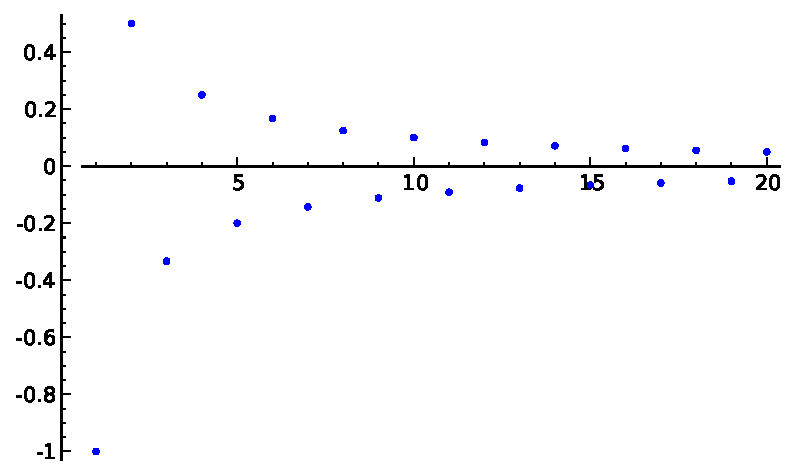
\includegraphics[width=9.5cm]{folge.pdf}
\end{center}

KONV KRIT

\begin{itemize}
\item Jede monotone, beschränkte Folge konvergiert.
\item Konvergenz bei Addition: Sind $(a_n)_n$ und $(b_n)_n$ konvergente Folgen, $\alpha, \beta \in \mathbb{R}$, so ist auch die
                   Folge $( \alpha a_n+\beta b_n)_n$ konvergent mit
                   dem Grenzwert
 \[ \lim_{n \rightarrow \infty} ( \alpha a_n + \beta b_n)= \alpha
                   \lim_{n \rightarrow \infty} a_n + \beta \lim_{n
                   \rightarrow \infty} b_n .\]
\item Konvergenz bei Multiplikation: Sind $(a_n)_n$ und $(b_n)_n$ konvergente Folgen, so ist auch die
                   Folge $(a_n b_n)_n$ konvergent mit
                   dem Grenzwert
 \[
  \lim_{n \rightarrow \infty} ( a_n b_n)= 
                   (\lim_{n \rightarrow \infty} a_n) \cdot  (\lim_{n
                   \rightarrow \infty} b_n).
 \]
\item Bemerkung: Weglassen oder Hinzufügen endlich vieler Glieder verändert das
                   Konvergenzverhalten nicht.
\end{itemize}

SÄTZE

\begin{itemize}
\item \emph{(Bolzano-Weierstrass)}: Jede beschränkte Folge besitzt (mindestens) eine
konvergente Teilfolge.
\item Jede Teilfolge einer konvergenten Folge konvergiert gegen den
Grenzwert der ursprünglichen Folge.
\item Jede konvergente Folge ist beschränkt, d.h. es gibt ein $K>0$,
so dass $|a_n|\leq K$ gilt für alle $n \in \mathbb{N}$.
\item \emph{Zwischenfolge}: Seien $(a_n)_n$ und $(b_n)_n$ konvergente Folgen mit $\lim_{n
\rightarrow \infty} a_n = \lim_{n \rightarrow \infty} b_n$. Dann gilt
für eine Folge $(c_n)_n$ mit $a_n \leq c_n \leq b_n$, $n \in
\mathbb{N}$, dass sie konvergiert mit  $\lim_{n
\rightarrow \infty} c_n = \lim_{n \rightarrow \infty} b_n$.
\end{itemize}

REK

Rekursive Folgen können durch rekursive Funktionen erzeugt werden.
\textbf{Beispiel:}
\[ y_{n+2}:=2y_{n+1}-y_n+2, \quad y_0=-1, y_1=a. \]
\begin{sagein}
var('a')
def y(n):
   if n==0:
       return -1
   if n==1:
       return a
   return 2*y(n-1)-y(n-2)+2
y(4)
\end{sagein}
\begin{sage}
4*a + 15
\end{sage}

%%%%%%%%%%%%%%%%%%%%%%%%%%%%%%%%%%%%%%
\section{Reihen}
%%%%%%%%%%%%%%%%%%%%%%%%%%%%%%%%%%%%%%
Sei $(a_n)_n$ eine Folge reeller Zahlen. Eine {\color{red} (unendliche)
Reihe} mit den {\color{red} Gliedern} $a_n$, in Zeichen
\[ \sum_{n=1}^\infty a_n =a_1 + a_2 + a_3 + \dots, \]
ist definiert durch die Folge $(s_n)_n$ der {\color{red} Partialsummen}\\
\[
s_n=\sum_{k=1}^n a_k = a_1+a_2+ \dots +a_n 
\]
Der Grenzwert $s$ der Folge $(s_n)_n$ wird als {\color{red} Wert} oder 
{\color{red} Summe} der Reihe bezeichnet. Man schreibt
\[s= \sum_{n=1}^\infty a_n.\] 

BEMERKUNGEN

\begin{itemize}
\item  Reihen sind eine spezielle Art von Folgen.
\item Indizierung mit $m$: $\sum_{n=m}^\infty a_n$.
\item Bei Abänderung, Weglassen oder Hinzufügen endlich vieler Glieder
bleiben Konvergenz und Divergenz unberührt. I.A. wird sich aber der
Grenzwert ändern.
\end{itemize}

inSAGE

\begin{sagein}
sum(<f>,<i>,<a>,<b>) 
\end{sagein}
Gesucht: geschlossene Darstellung der Summe $\sum_{i=a}^b f(i)$ mit $a,b \in \mathbb{Z}$ ganze
Zahlen (auch unendlich (\isage{infinity/oo}), \isage{f} Ausdruck in $i$.
\begin{itemize}
\item Oft ist die Konvergenz einer Reihe abhängig von bestimmten Parametern. Je nach Parameterwert zeigt die Reihe
unterschiedliches Konvergenzverhalten.
%geometrische Reihe z.b.
\end{itemize}

BEISPIELE

\begin{itemize}
\item \emph{geometrische Reihe}: $\sum_{n=0}^\infty x^n$. Die
Partialsummen lauten
\[ s_n=1+x+x^2+\ldots + x^n = \left \{ \begin{array}{ll}
n+1, & \mbox{ falls } x=1\\
\frac{1-x^{n+1}}{1-x}, & \mbox{ falls } x \neq 1 
\end{array} \right. .\]
Die Reihe divergiert für $|x|\geq1$ und konvergiert für $|x|<1$ mit
dem Wert $\sum_{n=0}^\infty = \frac{1}{1-x}$.

\begin{sagein}
sum(x^k,k,0,oo)
\end{sagein}
\begin{sage}
Is  abs(x)-1  positive, negative, or zero?
\end{sage}
Entsprechend gibt es keine geschlossene Form. Für $x=1/2$ gilt
\begin{sagein}
x = 1/2; sum(x^k,k,0,oo)
\end{sagein}
\begin{sage}
  2
\end{sage}
\item Die Reihe $\sum_{n=1}^\infty \frac{1}{n^2}$ konvergiert gegen
$\pi^2/6$.
\begin{sagein}
_=var('k');sum(1/k^2,k,1,oo)
\end{sagein}
\begin{sage}
1/6*pi^2
\end{sage}
\item Die \emph{alternierende harmonische Reihe}  $\sum_{n=1}^\infty
\frac{(-1)^{n+1}}{n}$ konvergiert.
\begin{sagein}
sum((-1)^(k+1)/k,k,1,oo)
\end{sagein}
\begin{sage}
  log(2)
\end{sage}
\item Die \emph{harmonische Reihe} $\sum_{n=1}^\infty \frac{1}{n}$
 divergiert.
\begin{sagein}
sum(1/k,k,1,oo)
\end{sagein}
\begin{sage}
ValueError: Sum is divergent
\end{sage}
\end{itemize}

PARTIALSUMMEN

\begin{itemize}
\item Definieren der Partialsumme
\begin{sagein}
_=var('x,n,k')
s = sum(x^k,k,0,n); s
\end{sagein}
{\color{blue}\[\frac{x^{{\left(n + 1\right)}} - 1}{x - 1}\]}
% \begin{sage}
% (x^(n + 1) - 1)/(x - 1)
% \end{sage}

\item Die ersten $5$ Glieder der Partialsumme
\begin{sagein}
assume(x<>1); [s(n=m) for m in [1..6]]
\end{sagein}
{\color{blue}\[\left[\frac{x^{2} - 1}{x - 1}, \frac{x^{3} - 1}{x - 1}, \frac{x^{4} - 1}{x - 1}, \frac{x^{5} - 1}{x - 1}, \frac{x^{6} - 1}{x - 1}, \frac{x^{7} - 1}{x - 1}\right] \]}
% \begin{sage}
% [(x^2 - 1)/(x - 1), (x^3 - 1)/(x - 1), (x^4 - 1)/(x - 1), (x^5 - 1)/(x -
% 1), (x^6 - 1)/(x - 1), (x^7 - 1)/(x - 1)]
% \end{sage} 
\item Bestimmen des Grenzwertes der Folge der Partialsummen
\begin{sagein}
forget();assume(abs(x)<1);limit(s,n=oo)
\end{sagein}
\begin{sage}
-1/(x - 1)
\end{sage}
\begin{sagein}
forget();assume(x>1);limit(s,n=oo)
\end{sagein}
\begin{sage}
+Infinity
\end{sage}
 \end{itemize}

assume()

\begin{sagein}
assume(<assumptions>)
\end{sagein}
Annahmen für bestimmte Bezeichner.

\textbf{Beispiele:}
\begin{sagein}
assume(x,'real') # §$x$§ wird auf §$\mathbb{R}$§ eingeschränkt
assume(x>a) # §$x$§ wird auf  §$\{y \in \mathbb{R}\ |\ y>a\}$§ eingeschränkt
\end{sagein}

Ruft man \isage{assume} mehrmals für einen Bezeichner auf, werden zusätzliche Annahmen gemacht. Sind diese
Widersprüchlich erhält man eine entsprechende Meldung.

BEMERKUNGEN

\begin{itemize}
\item Umformungen oder Vereinfachungen für symbolische Bezeichner
werden i.A. nur dann durchgeführt,
wenn sie für alle komplexen Zahlen gelten. Hier kann ein Einschränken
des Definitionsbereichs helfen.
\item Mittels 
\begin{sagein}
forget(x>a)
\end{sagein}
wird die Annahme \isage{x>a} gelöscht.
\item Durch 
\begin{sagein}
assumptions() 
\end{sagein}
können alle Annahmen ausgegeben werden.
%\item Durch den speziellen Bezeichner \isage{Global} können Annahmen
%für alle Bezeichner gesteuert werden. 
\end{itemize}

BEISPIELE

\begin{sagein}
var('c'); assumptions()
\end{sagein}
\begin{sage}
c
[]
\end{sage}

\begin{sagein}
c = 2; assume(c>0)
\end{sagein}
\begin{sage}
 AttributeError: 'bool' object has no attribute 'assume'
\end{sage}
\begin{sagein}
_=var('c')
assume(c,'integer'); assumptions()
\end{sagein}
\begin{sage}
[c is integer]
\end{sage}
\begin{sagein}
sin(c*pi)
\end{sagein}
\begin{sage}
sin(pi*c)
\end{sage}
\begin{sagein}
sin(c*pi).simplify()
\end{sagein}
\begin{sage}
   0
\end{sage}
\begin{sagein}
assume(x>0)
sqrt(x^2).simplify()
\end{sagein}
\begin{sage}
  x
\end{sage}


% integer,
% noninteger, even, odd, rational, irrational, real, imaginary, complex,
% analytic, increasing, decreasing, oddfun, evenfun, posfun, constant,
% commutative, lassociative, rassociative, symmetric, antisymmetric,
% integervalued, one_to_one
\begin{center}
 \begin{tabular}{|l|l|}
\hline
Annahme & Erklärung\\
\hline
\isage{'real'} & $\mathbb{R}$ \\
\isage{'rational'} & $\mathbb{Q}$\\
\isage{'integer'} &  $\mathbb{Z}$\\
\isage{'complex'} & $\mathbb{C}$\\
\isage{'even'}   & gerade Zahl \\
\isage{'odd'} & ungerade Zahl\\
\isage{'increasing'} & wachsend \\
\isage{'analytic'} & analytisch\\
\hline
\end{tabular}
\end{center}

KONV KRIT

\begin{itemize}
\item \emph{Cauchykriterium:} Eine Reihe $\sum_{n=1}^\infty a_n$ konvergiert
                  genau dann, wenn es zu jedem $\varepsilon>0$ ein $n_0
                  \in \mathbb{N}$ gibt, so dass für alle $m,n \geq n_0$
                  gilt $| \sum_{k=m}^n a_k|<\varepsilon$.
\item \emph{Notwendiges Kriterium:} Konvergiert eine Reihe, so bilden ihre Glieder eine Nullfolge. Dieses Kriterium ist \emph{nicht} hinreichend!
\item \emph{Verdichtungskriterium:} Eine Reihe $\sum_{n=1}^\infty a_n$ mit
                  einer Folge nichtnegativer, monoton fallender
                  Glieder konvergiert genau dann, wenn die Reihe
                  $\sum_{n=1}^\infty 2^n a_{2^n}$ konvergiert.
\end{itemize}
Gilt $0 \leq c_n \leq a_n \leq b_n$ für alle $n \in \mathbb{N}$
\begin{itemize}
 \item {\color{red} Minorante}: $\sum_{n=1}^\infty c_n$
 \item {\color{red} Majorante}: $\sum_{n=1}^\infty b_n$ 
\end{itemize}
Die Reihe $\sum_{n=1}^\infty a_n$ \emph{konvergiert}, wenn...
\begin{description}
\item[Majorantenkriterium:] eine konvergente Majorante besitzt (nichtnegative Glieder).

\item[Quotientenkriterium:] Die Glieder positiv sind und ein $q<1$
existiert, so dass für $n \in \mathbb{N}$ gilt $\frac{a_{n+1}}{a_n}
\leq q$. 
\item[Wurzelkriterium:] Die Glieder positiv sind und ein $q<1$
existiert, so dass für $n \in \mathbb{N}$ gilt $\sqrt[n]{a_n} \leq
q$. 
\item[Leibnizsches Kriterium:] wenn die Folge $(a_n)_n$ bei $\sum_{n=1}^\infty (-1)^n a_n$
eine monoton fallende  Nullfolge ist.
\end{description}
Die Reihe $\sum_{n=1}^\infty a_n$ \emph{divergiert}, wenn...
\begin{description}
\item[Majorantenkriterium:] sie eine divergente Minorante besitzt.
\end{description}

BEISPIELE

\begin{itemize}
\item Betrachte $\sum_{n=0}^\infty n^4 e^{-n^2}$
\begin{sagein}
f(n) = n^4*exp(-n*n)
g(n) = f(n+1)/f(n)
limit(g(n),n=oo)
\end{sagein}
\begin{sage}
  0
\end{sage}
\item Betrache $\sum_{n=2}^\infty \frac{1}{n (\log n)^2}$
\begin{sagein}
f(n) = 1/(n*(log(n)^2))
g(n) = 2^n*f(2^n)
h(n) = 2^n*g(2^n)
limit(h(n+1)/h(n),n=oo)
\end{sagein}
\begin{sage}
  1/2
 \end{sage}
\end{itemize}

ABS BED KONV

{\color{red} absolut konvergent}: Ist eine Reihe $\sum_{n=0}^\infty a_n$ 
genau dann wenn $\sum_{n=0}^\infty |a_n|$ konvergiert. 

{\color{red} bedingt konvergent}: konvergent, aber nicht absolut konvergent.
\begin{itemize}
\item Absolut konvergente Reihen können beliebig umgeordnet werden.
\item Dies ist i.d.R. bei nicht absolut konvergenten Reihen falsch!
\end{itemize}

%%%%%%%%%%%%%%%%%%%%%%%%%%%%%%%%%%%%%%
\section{Potenzreihen}
%%%%%%%%%%%%%%%%%%%%%%%%%%%%%%%%%%%%%%
{\color{red} Potenzreihe}:
\[ \sum_{n=0}^\infty a_n (x-x_0)^n \]
mit $x_0 \in \mathbb{R}$. 

{\color{red} Konvergenzradius}: 
\[  \rho := \frac{1}{ \limsup_{n \rightarrow \infty} \sqrt[n]{|a_n|}}
\]
Ist $a_n \neq 0$ für alle $n > n_0$:
\[
 \rho = \limsup_{n \rightarrow \infty} \frac{|a_{n}|}{|a_{n+1}|}.
\]

Konvergenzverhalten:
\begin{itemize}
 \item konvergiert absolut für $|x -x_0|< \rho$.
 \item divergiert für $|x-x_0|>\rho$.
\item Die Konvergenz an den Stellen $x_0-\rho$ und $x_0+\rho$ muss bei
jeder Reihe individuell geprüft werden.   
\end{itemize}

BEISPIELE

\begin{itemize}
\item $\sum_{n=1}^\infty \frac{x^n}{n!}$
\begin{sagein}
f(n) = 1/factorial(n)
rho = limit(expand(f(n)/f(n+1)),n=oo); rho
\end{sagein}
\begin{sage}
+Infinity
\end{sage}
Die Potenzreihe konvergiert für alle $x \in \mathbb{R}$. 
\item $\sum_{n=0}^\infty n^s x^n$, $s>0$
\begin{sagein}
_=var('s');f(n)= n^s; assume(s>0)
limit(expand(f(n)^(1/n)),n=infinity)
\end{sagein}
\begin{sage}
  1
\end{sage}
Der Konvergenzradius ist $1$.
\end{itemize}

EXP

Wir erklären die \emph{Exponentialfunktion} durch
\[  exp(x) := \sum_{i=0}^\infty \frac{x^n}{n!}= 1 + \frac{x}{1!} +
\frac{x^2}{2!}+ \frac{x^3}{3!}+ \dots, x \in \mathbb{R}. \]
 Die Funktion ist auf ganz $\mathbb{R}$ definiert. Plot:
\begin{sagein}
plot(exp,(-5,5))
\end{sagein}
\begin{center}
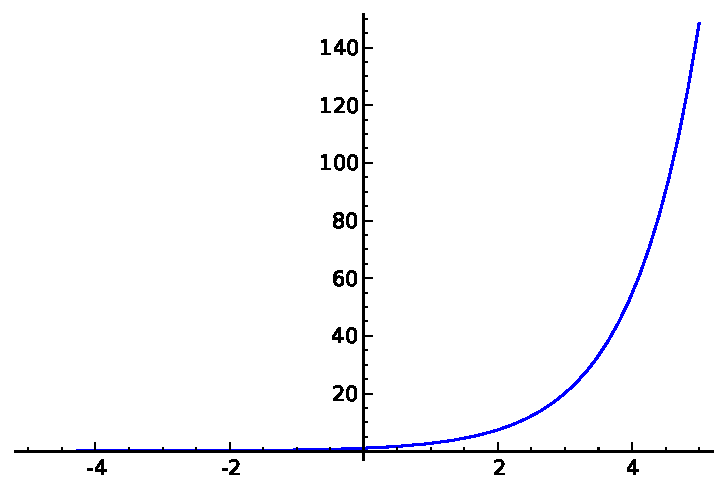
\includegraphics[width=6cm]{fexp.pdf}
\end{center}

EIG EXP

\begin{itemize}
\item Es gilt $\exp(x+y)=\exp(x) \cdot \exp(y)$.
\item Es gilt $\exp(x)=\lim_{n \rightarrow \infty} (1+\frac{x}{n})^n$.
\item Es gilt $\exp(x)=1/\exp(-x)$.
\item Die Umkehrfunktion auf $\mathbb{R}_+$ der Exponentialfunktion ist die
Logarithmusfunktion $\log (x)$. Es gilt
\[ \exp(\log(x))=x, \ x >0, \quad \log ( \exp ( x ))=x, \ x \in \mathbb{R}.\] 
\item Die {\color{red} allgemeine Potenz} ist durch $a^x:=\exp( x \log a)$,
$a\in \mathbb{R}_+$
definiert. 
\end{itemize}

inSAGE

\begin{sagein}
sum(x^n/factorial(n),n,0,oo)
\end{sagein}
\begin{sage}
  e^x
\end{sage}
\begin{sagein}
exp(log(x))
\end{sagein}
\begin{sage}
  x
\end{sage}
\begin{sagein}
_=var('n');limit((1+x/n)^n,n=oo)
\end{sagein}
\begin{sage}
  e^x
\end{sage}
% \begin{sagein}
% ??
% ??
% \end{sagein}
% \begin{sage}
%   
% \end{sage}

TRIG

Die {\color{red} Sinusfunktion} und die {\color{red} Cosinusfunktion} sind definiert
durch
\begin{eqnarray*}
\sin(x) := \sum_{n=0}^\infty (-1)^n \frac{x^{2n+1}}{(2n+1)!} \quad\quad
\cos(x) := \sum_{n=0}^\infty (-1)^n \frac{x^{2n}}{(2n)!}. 
\end{eqnarray*}
Die Potenzreihen konvergieren für alle $x \in \mathbb{R}$. Plotten:
\begin{sagein}
p = plot(sin,0,4*pi,color='red')
p += plot(cos,0,4*pi); 
p += text('-- $\sin(x)$', (10, 1.0), color='red')
p += text('-- $\cos(x)$', (10, 0.85)); p.show()
\end{sagein}
\begin{center}
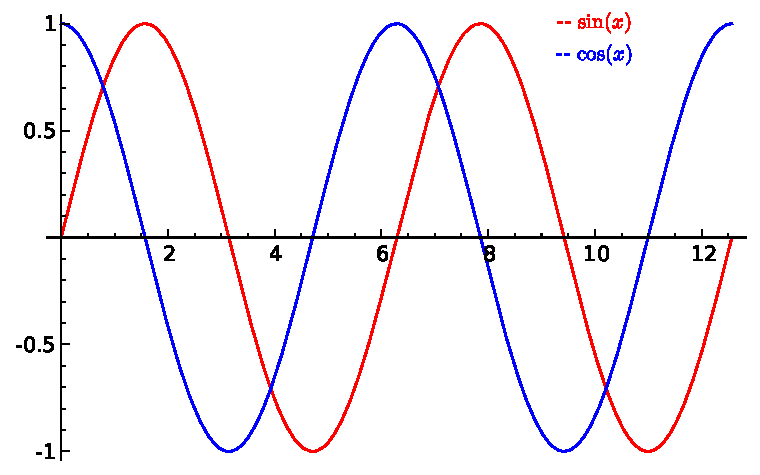
\includegraphics[width=5.5cm]{sincos.pdf}
\end{center}

EIG TRIG

\begin{itemize}
\item \emph{Additionstheoreme}:
\begin{eqnarray*}
\sin(x+y) & = &\sin x \cos y+ \cos x \sin y \\
\cos(x+y) & = &\cos x \cos y - \sin x \sin y .
\end{eqnarray*} 
\item 
\[\sin^2x +\cos^2x=1.\]
\item 
\begin{eqnarray*}
\sin(x+\pi/2)&=&\cos(x)\\
 \cos(x+\pi/2)&=&-\sin(x).
\end{eqnarray*} 
\item Wir definieren $\pi$, indem wir die kleinste positive Nullstelle
von $\cos(x)$ als $\pi/2$ definieren.

\end{itemize}

inSAGE

\begin{sagein}
solve(cos(x)==0,x)
\end{sagein}
\begin{sage}
[x == 1/2*pi]
\end{sage}
\begin{sagein}
sin(x+pi/2).simplify()
\end{sagein}
\begin{sage}
cos(x)
\end{sage}

MORE EIG

\begin{itemize}
%\item Man kann die Sinusfunktion und die Cosinusfunktion mit Hilfe eines rechtwinkligen Dreiecks im Einheitskreis auch geometrisch  deuten.
\item Umkehrfunktionen: $\arcsin$ bei Sinus und $\arccos$ bei Cosinus.
Plotten: 
\begin{sagein}
p = plot(arcsin,-1,1,color='red')
p += plot(arccos,-1,1); 
p += text('-- arcsin(x)', (-0.7, 1.0), color='red')
p += text('-- arccos(x)', (-0.7, 0.75)); p.show()
\end{sagein}
\begin{center}
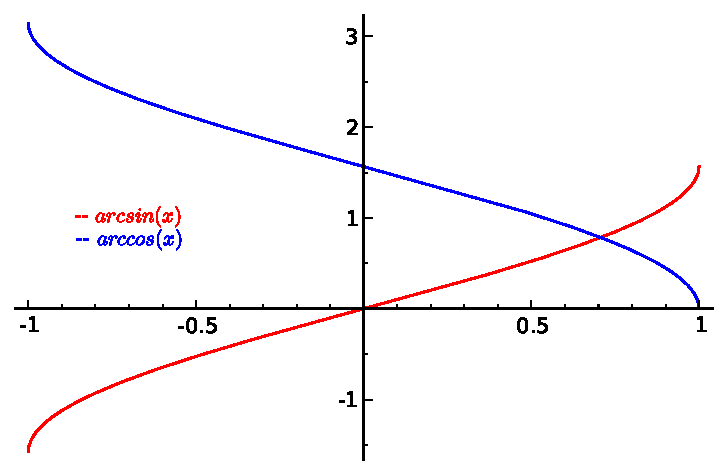
\includegraphics[width=6.5cm]{arcsinarccos.pdf}
\end{center}
\item Der {\color{red} Tangens} ist definiert durch
$\tan(x) :=\frac{\sin(x)}{\cos(x)}$.
\begin{sagein}
plot(tan,-4,4,detect_poles=True,ymax=4,ymin=-4)
\end{sagein}
\begin{center}
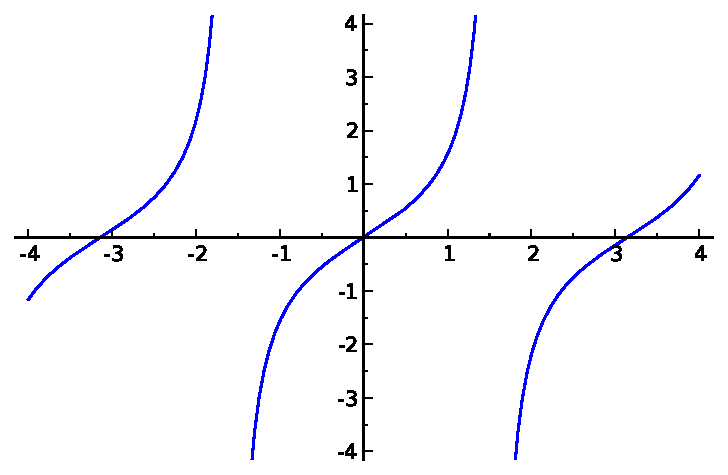
\includegraphics[width=7cm]{tan.pdf}
\end{center}
\end{itemize}

%%%%%%%%%%%%%%%%%%%%%%%%%%%%%%%%%%%%%%
\section{Vertiefung Schleifen}
%%%%%%%%%%%%%%%%%%%%%%%%%%%%%%%%%%%%%%

WHILE

\begin{sagein}
while <expression> :
    <Code-block>
\end{sagein}
Diese wiederholt \isage{<Code-block>} solange wie die \isage{<expression>} als 
\isage{True} ausgewertet wird.

\textbf{Beispiel}:
\begin{sagein}
f(x) = 1/x
x=0.1
while f(x) > 0.1:
    x += 0.1
x
\end{sagein}
\begin{sage}
 10.1000000000000
\end{sage}
%achtung: rundungsfehler, daher kommt 10.1 raus.. selbst einmal drauf reingefallen..

% \begin{itemize}
% \item Die Schleifenvariable $k$ durchläuft die Werte $1$, $2$, $3$ und
%   $4$. Dabei wird alles was ab \isage{:} eingerückt ist $k$-mal durchlaufen.
% \item Ergebnisse, die in jedem Schleifenschritt berechnet werden,
%   werden \alert{nicht} auf dem Bildschirm ausgegeben. 
% \item Eine Ausgabe wird durch den \isage{print}-Befehl erzielt.
% \end{itemize}
% \end{frame}

% \begin{frame}[fragile]{Schleifen III}
%  Eine elegante Möglichkeit sind Schleifen über Listen oder Mengen.
% \begin{sage}
% L = [1..10]
% for i in L:
%     x = i^2
%     print("Das Quadrat von {0} ist {1}").format(i,x)
% \end{sage}
% \end{frame}


% \begin{frame}[fragile]{Etwas Zahlentheorie}
% Wir geben für die natürlichen Zahlen $\leq 1000$ an, wieviele Zahlen
% $1,2,3,\dots $ Teiler haben.
% \begin{sagein}
% Liste = [1..1000]
% def anz_teiler(n): return len(divisors(n))
% Liste2 = map(anz_teiler,Liste)
% for k in [1..50]:
%     print "{0} , {1}".format(k,len(filter(lambda x: x == k, Liste2)))
% print divisors(840)
% \end{sagein}

ALT

\begin{itemize}
\item Schleifen abwärts zählen
\begin{sagein}
for j in reversed([2,4]):
   print("{0}, {1}").format(x,x^j) 
\end{sagein}
\item Schrittweite modifizieren
\begin{sagein}
for j in srange(3,10,2.6):
    print(x,x^j) 
\end{sagein}
\begin{sage}
(x, x^3.00000000000000)
(x, x^5.60000000000000)
(x, x^8.20000000000000)
\end{sage}

\end{itemize}

FP

Suche ein $x_{\mathrm{fix}} \in \mathbb{R}$ so dass
\[ x_{\mathrm{fix}} = \cos (x_{\mathrm{fix}}) \]
gilt.
\begin{center}
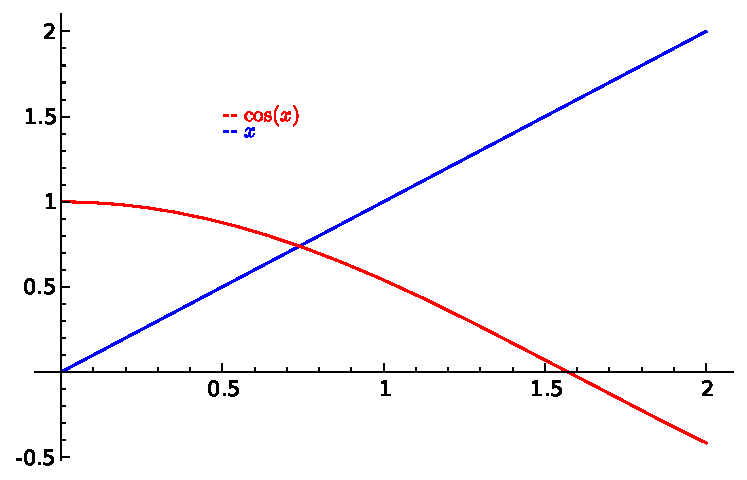
\includegraphics[width=8cm]{iter1.pdf}
\end{center}

FP-IT

Fixpunkt-Iteration 
\[ x_{k+1}=cos(x_k) \]
bei geeignetem Startwert $x_0 = 0.2$.  \\
\centering{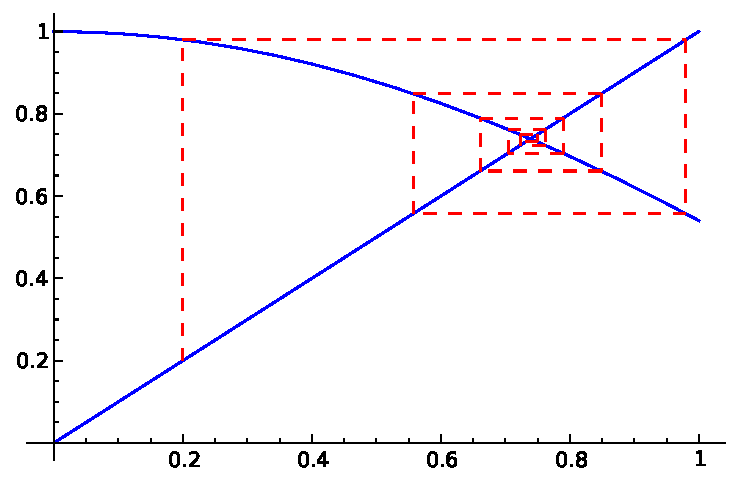
\includegraphics[width=8cm]{fixpunkt.pdf}}\\

IMP

\begin{small}
\begin{sagein}
def fixpunkt(f,In,x0,n):
    y = [x0]
    p = plot(f,(In[0],In[1]))
    p += plot(x,(In[0],In[1]))
    for i in [0..n-1]:
        y.append(float(f(y[i])))
        p += line( [ (y[i],y[i]), (y[i],y[i+1]) ],linestyle='--', color='red')
        p += line( [ (y[i],y[i+1]), (y[i+1],y[i+1]) ],linestyle='--', color='red')
    p.show()
    return(y)
\end{sagein}
\end{small}

CALL

\begin{sagein}
fixpunkt(lambda x: cos(x),[0,1],0.2,10)
\end{sagein}
\begin{sage}
[0.200000000000000, 0.98006657784124163, 0.55696725280964243, 0.84886216565827077, 0.66083755111661502, 0.78947843776686832, 0.70421571334199318, 0.76211956176066087, 0.72337417210557109, 0.74957657633149311, 0.73197742525819132]
\end{sage}







\end{document}